\documentclass[a5paper,openany]{book}


\usepackage[utf8]{inputenc}
\usepackage[T1]{fontenc}
\usepackage[english]{babel}

% set font to Linux Libertine (non-proprietary font):
% this requires downloading the font, e.g., from
%    https://sourceforge.net/projects/linuxlibertine/
% and installing it manually
% then, compile using xelatex paperwriting.tex
% \usepackage{fontspec}
% \setmainfont{Linux Libertine O}
% alternative for pdflatex (does not work with certain font variants)
\usepackage{libertine}

%\usepackage[pass]{geometry}  % to make a5paper work
\usepackage[a5paper,bottom=3cm]{geometry}

\usepackage{setspace}
\setstretch{1.2}  % default value: 1.44

% \usepackage{tocloft}

\usepackage{mathtools,amsfonts}  % for math (loads amsmath, amsfonts(?), amssymb)
\usepackage{aligned-overset}  % for aligned overset

\usepackage{pifont}  % for checkmark, cross
\usepackage{siunitx}  % for SI units guideline

\usepackage{xcolor}  % customized colors
\usepackage[most]{tcolorbox}  % for guidelines and examples, loads tikz
\tcbuselibrary{skins}  % enhanced formatting for tcolorbox
\tcbuselibrary{raster}  % for good/bad examples

\usepackage{pgfplots}
\usepgfplotslibrary{groupplots}
\usetikzlibrary{arrows,patterns}

\usepackage{enumitem}  % lists (currently, modifying items)
\setlist[itemize]{itemsep=0pt, left=8pt}

\usepackage{algpseudocode}  % algorithmic environment

\usepackage{booktabs}  % tables
\usepackage{multirow}  % tables
% \usepackage{longtable}  % for table of references for guidelines

\usepackage{soul}  % for highlighting multiline text

\usepackage{fancyhdr}  % for formatting headers
\pagestyle{fancy}  % enable custom header functionality
\renewcommand{\headrulewidth}{0pt}  % no horizontal line below header

\fancyhead[L]{\thepage}  % left header: page number
\fancyhead[C]{}
\fancyhead[R]{\nouppercase{\leftmark}}  % right header: chapter number and name
\fancyfoot[L]{}
\fancyfoot[C]{}
\fancyfoot[R]{}

% glossary / list of terms
% \usepackage[nopostdot]{glossaries}
% \newglossaryentry{emphasis}{name = {emphasis}, description={}}
%% \setglossarystyle{list}
%% \makeglossaries


\usepackage{csquotes}  % required by compilation?
\usepackage[backend=biber,
    url=false,
    doi=true,
    isbn=true,
    style=ext-numeric-comp,
    defernumbers=true,
    %giveninits,
    sorting=none,
    maxnames=100]{biblatex}
\addbibresource{tex/references.bib}

\DeclareFieldFormat{titlecase:title}{\MakeSentenceCase*{#1}}
\DeclareFieldFormat{titlecase:booktitle}{#1}
\DeclareFieldFormat{titlecase:journaltitle}{#1}
\DeclareFieldFormat{doi}{doi: \text{#1}}

% colors for boxes
\definecolor{color_guideline}{RGB}{0, 92, 171}
\definecolor{color_guideline_background}{rgb}{0.588, 0.784, 0.902}
\definecolor{color_example_frame}{rgb}{0.65,0.65,0.65}
\definecolor{color_highlight}{RGB}{255, 195, 37}
% \definecolor{color_example_good}{rgb}{0.4706,0.7725,0.4980}
% \definecolor{color_example_bad}{rgb}{0.9059,0.7373,0.7373}

\definecolor{color_example_good}{HTML}{228B22}
\definecolor{color_example_bad}{HTML}{B22222}

% guidelines
\newcounter{guidelinecounter}
\newcommand{\guideline}[3][defaultguidelinelabel]{%
\refstepcounter{guidelinecounter}
\label{#1}
\begin{tcolorbox}[
    title=Guideline \theguidelinecounter.,
    colback=color_guideline_background, colframe=color_guideline,
    sharp corners=northwest,bottomrule=0mm,rightrule=0mm,leftrule=0mm,
    left=2mm,right=2mm]
    #2
\end{tcolorbox}%
\addcontentsline{toc}{section}{Guideline \theguidelinecounter. #2}
}

% text example for comparison good/bad (two columns)
\newcommand{\goodbadexample}[3][]{%
\ifx\relax#1\relax
\begin{tcbraster}[raster row skip=3pt,raster columns=1]
\begin{tcolorbox}[enhanced,breakable,frame hidden,interior hidden,colback=white,
    borderline west={0.75mm}{0.25mm}{color_example_bad},
    top=0mm,bottom=0mm,right=0mm,left=2.5mm]
    #2
\end{tcolorbox}
\begin{tcolorbox}[enhanced,frame hidden,interior hidden,colback=white,
    borderline west={0.75mm}{0.25mm}{color_guideline},
    top=0mm,bottom=0mm,right=0mm,left=2.5mm]
    #3
\end{tcolorbox}%
\end{tcbraster}%
\else
{\hfill \scriptsize{#1}}
\begin{tcbraster}[raster before skip=0pt,raster row skip=3pt,raster columns=1]
\begin{tcolorbox}[enhanced,breakable,frame hidden,interior hidden,colback=white,
    borderline west={0.75mm}{0.25mm}{color_example_bad},
    top=0mm,bottom=0mm,right=0mm,left=2.5mm]
    #2
\end{tcolorbox}
\begin{tcolorbox}[enhanced,frame hidden,interior hidden,colback=white,
    borderline west={0.75mm}{0.25mm}{color_guideline},
    top=0mm,bottom=0mm,right=0mm,left=2.5mm]
    #3
\end{tcolorbox}%
\end{tcbraster}%
\fi%
}

% text example (single column)
\newcommand{\badexample}[2][]{%
\ifx\relax#1\relax
\begin{tcolorbox}[enhanced,breakable,frame hidden,interior hidden,colback=white,
    borderline west={0.75mm}{0.25mm}{color_example_bad},
    top=0mm,bottom=0mm,right=0mm,left=2.5mm]
    #2
\end{tcolorbox}%
\else
{\hfill \scriptsize{#1}}
\begin{tcolorbox}[before skip=0pt,
    enhanced,breakable,frame hidden,interior hidden,colback=white,
    borderline west={0.75mm}{0.25mm}{color_example_bad},
    top=0mm,bottom=0mm,right=0mm,left=2.5mm]
    #2
\end{tcolorbox}%
\fi%
}
\newcommand{\goodexample}[2][]{%
\ifx\relax#1\relax
\begin{tcolorbox}[enhanced,breakable,frame hidden,interior hidden,colback=white,
    borderline west={0.75mm}{0.25mm}{color_guideline},
    top=0mm,bottom=0mm,right=0mm,left=2.5mm]
    #2
\end{tcolorbox}%
\else
{\hfill \scriptsize{#1}}
\begin{tcolorbox}[before skip=0pt,
    enhanced,breakable,frame hidden,interior hidden,colback=white,
    borderline west={0.75mm}{0.25mm}{color_guideline},
    top=0mm,bottom=0mm,right=0mm,left=2.5mm]
    #2
\end{tcolorbox}%
\fi%
}

% highlight background of crucial parts
\sethlcolor{color_highlight}
\newcommand{\highlightpart}[1]{\hl{#1}}
\newcommand{\highlightempty}{\hl{ }}
\newcommand{\highlightpartmath}[1]{\text{\highlightpart{$#1$}}}  % soul can run into problems in math env

% row in table of references for guidelines
\newcommand{\guidelineref}[2]{\ref{#1} & \fullcite{#2} \\}


% command 'widecheck' for inner-approximations
\makeatletter
\DeclareRobustCommand\widecheckinternal[1]{{\mathpalette\@widecheckinternal{#1}}}
\def\@widecheckinternal#1#2{%
	\setbox\z@\hbox{\m@th$#1#2$}%
	\setbox\tw@\hbox{\m@th$#1%
		\widehat{\vrule\@width\z@\@height\ht\z@
			\vrule\@height\z@\@width\wd\z@}$}%
	\dp\tw@-2\ht\z@
	%	\dp\tw@-\ht\z@
	\@tempdima\ht\z@ \advance\@tempdima2\ht\tw@ \divide\@tempdima\thr@@
	%	\setbox\tw@\hbox{\raise\@tempdima\hbox{\scalebox{1}[-1]{\lower\@tempdima\box\tw@}}}%
	\setbox\tw@\hbox{\raise1.05\@tempdima\hbox{\scalebox{1}[-1]{\lower\@tempdima\box\tw@}}}%
	{\ooalign{\box\tw@ \cr \box\z@}}}
\makeatother
\newcommand{\widecheck}[1]{\,\widecheckinternal{\kern -2pt #1}}

% indication of sections
\newcommand{\location}[1]{\begin{footnotesize} (\textsc{#1}) \end{footnotesize}}

%%%% titlepage
\title{\huge Guidelines for Scientific Paper Writing in Computer Science}
\author{\Large Mark Wetzlinger}
\date{}
%%%%


\begin{document}

%%%% TITLE, ACKS, PREFACE, TOC %%%%
\frontmatter

\maketitle

\chapter*{Acknowledgments}

First and foremost, I want to express my gratitude to my advisor Matthias and my mentor Niklas, who taught me most of what I know.
Many thanks also to my wonderful group of colleagues, and in particular Hanna, for mutual proofreading over many years as well as countless discussions on the craft of paper writing.
% TODO: Include proofreaders, e.g.: Special thanks to ... for proofreading early versions.

% \bigskip

% \noindent Munich, November 2024 \hfill Mark Wetzlinger%

\chapter*{Preface}

Publishing papers is the main task in pursuing a doctoral degree.
This task can be split in two stages: conducting research and writing papers.
The difference between the two stages lies in the qualities required for success.
Conducting research is more akin to art, with an emphasis on creativity and ingenuity to generate novel ideas and tackle unsolved problems.
In contrast, paper writing is a craft, with a focus on technical proficiency, attention to detail, and precision in execution.

I was very fortunate to have had both a PhD supervisor and a mentor that invested time and efforts in teaching me this craft.
Besides writing papers myself, I have also proofread numerous drafts of my junior colleagues, and I have reviewed many submissions to conference proceedings and journals.
The feedback loop between writing your own work and reviewing the work of others is essential for developing good writing skills.
Reading and reviewing papers allows you to consciously reflect on what makes a paper appealing to the reader.
Still, no skill can be attained without sufficient hands-on practice.
Hence, the true learning happens when you are forced to make decisions in your own work.

After more than five years of making such decisions, I believe to have understood a thing or two about the craft of paper writing.
Of course, it would be presumptuous to claim there were one way of writing a literature review, presenting a novel approach, or discussing numerical results.
Yet, one can discuss the how-to on an abstract level and provide generic advice applicable in many cases.
I have gained this conviction through repeatedly making the same suggestions for improvement during review.
And so, I have decided to comprise my knowledge and observations in this booklet.
The word ``guidelines'' in the title is carefully chosen, as there is no one truth but only a path towards it.
Some guidelines may be more contentious than others, but I believe any such discussion on the authors' side is ultimately in the best interest of the readers.

A few brief words on the content and its presentation:
The booklet is split into two parts---the first part offers guidelines on the level of sections and paragraphs,
while the second part addresses questions on the level of individual sentences and words.
For each guideline, we first provide a concise formulation, then present an example, and finally offer a brief explanation.
Examples are either a comparison between a preferable version and its disadvantageous counterpart or only show a possible implementation of the guideline.
The key parts in the examples are highlighted, unless there is no identifiable key part, usually because the example as a whole illustrates the guideline.
Furthermore, all examples are taken and/or adapted from my own papers;
where I could not find a fitting example, I have taken the liberty of constructing an example.

Let me conclude by restricting the scope of this booklet.
We specifically target the writing of regular papers, which explicitly excludes survey papers, tool papers, and benchmark papers, among others.
Still, I am convinced that many guidelines are applicable to those other types of papers, too.
Moreover, the scope is conservatively limited to computer science, as each research discipline has its own particularities in presenting their work.
I do hope, however, that much of the content is transferable to other research disciplines as well.

\bigskip

\noindent Thank you for reading, \\
\noindent Mark


%% standard table of contents
\tableofcontents

%% brief contents and standard table of contents
% \clearpage

% \setcounter{tocdepth}{0}
% \renewcommand{\contentsname}{Brief Contents}
% \setlength{\cftbeforepartskip}{10pt}
% \setlength{\cftbeforechapskip}{2pt}
% \tableofcontents
% \setlength{\cftbeforechapskip}{3pt plus 1pt minus 1pt}
% \setlength{\cftbeforepartskip}{10pt plus 2pt minus 2pt}

% \clearpage

% \setcounter{tocdepth}{1}
% \renewcommand{\contentsname}{Contents}
% \chapter*{\contentsname}
% \begingroup
%   \makeatletter
%   \input{paperwriting_longtoc.toc} % manually copied
%   \makeatother
% \endgroup

%% end


%%%% MAIN %%%%
\mainmatter

%%%% GOLDEN RULE %%%%

\chapter*{The Golden Rule}
\label{ch:consistency}
\addcontentsline{toc}{chapter}{The Golden Rule}

The title of this booklet explicitly mentions guidelines, which are flexible and context-dependent.
So why start with something as rigid as a rule?

Paper writing consists of making decisions about individual parts that ultimately compose a whole.
Each paper has its own needs:
Some report theoretical findings, others focus on the experimental evaluation;
some propose novel algorithms, others combine existing approaches to harness the respective advantages.
Therefore, generic statements about paper writing must be flexible enough to accommodate these different contexts.
Unfortunately, the increased generality correlates with an irrevocable loss in meaning.
Statements like \emph{'think about the story you want to tell'} or \emph{'clearly state your contribution'} are as true as they are useless---they are condensed to the point of being meaningless, and the original intent is irretrievable.

There is, however, one statement that defies the above analysis, being remarkably short but completely unequivocal.
It is applicable to works of all formats and topics, and adhering to it will always improve the work:

\begin{tcolorbox}[
    title=The Golden Rule.,
    colback=color_guideline_background, colframe=color_guideline,
    sharp corners=northwest,bottomrule=0mm,rightrule=0mm,leftrule=0mm]
    \textbf{Be consistent.}
\end{tcolorbox}

\noindent Personally, I consider the Golden Rule the single most important statement about scientific paper writing.

In general, consistency is established through a one-to-one correspondence between entities:
On a structural level, the title of each section must correspond to its content.
A section entitled \emph{discussion} provides a critical assessment of the presented work, potentially in comparison to related work; thus, no such assessments or comparisons should be made prior to or after this section.
On a wording level, one should use scientific terms consistently and avoid using different terms to refer to the same entity.
If the term \emph{model} refers to a specific mathematical formulation for a real-world phenomenon, then any such phenomenon should always be described using the term \emph{model}, and not by alternatives like \emph{system}.
On a mathematical level, variables should be used consistently throughout the paper to facilitate switching back and forth between different sections, such as the problem statement and the evaluation section.
More precisely, a variable like $x$ should consistently have the same meaning, and anything else than that must not be called $x$.

Ultimately, consistency establishes a level of trust between the author and the reader.
It helps in avoiding misunderstandings between the author's intent and the reader's understanding.
Many guidelines in the remainder of this booklet are mere applications of the Golden Rule in specific contexts.



%%%% HIGH LEVEL %%%%
\part{Organization and Structure}


\chapter{Abstract}
\label{ch:abstract}

The abstract provides a concise summary of the paper:
In order, it motivates and states the research question, highlights the limitations of existing methods, presents the main approach and its advantages, discusses the results of the evaluation, and provides a brief conclusion.
A well-written abstract helps readers quickly determine the paper's relevance to their interests.


\guideline{...}
% - start out with a sentence that sets a frame for the topic of the paper, why it is important, and can be understood by a broad audience

\goodbadexample{
    ...
}{
    ...
}

\noindent ...


\guideline[g:abstract:research_question]
    {State the research question addressed in your paper.}

\goodexample[{\cite[Abstract]{Wetzlinger2024CSL}}]{
    Inner approximations of the exact reachable set contain \highlightpart{only states that are definitely reachable} and are therefore \highlightpart{used to falsify specifications}.
}

\noindent
The next sentence(s) narrow down the general frame opened by the first sentence by concretizing the overarching research field to the specific topic of the paper.


\guideline[g:abstract:outline_limitations]
    {Outline the limitations of the state of the art.}

\goodexample[{\cite[Abstract]{Wetzlinger2024CSL}}]{
    While the majority of state-of-the-art approaches for nonlinear systems obtain an \highlightpart{inner approximation via first computing an outer approximation} of the reachable set, (...)
}

\noindent
Following the concretization of the topic, introduce the key motivation for your proposed contribution via a succinct overview of the state of the art.
For example, the specific research question has not yet been addressed, current approaches do not provide good results or do not scale well.
Crucially, the mentioned limitation(s) should directly lead to the next sentence, which summarizes the proposed contribution.


\guideline[g:abstract:summarize_approach]
    {Summarize the key steps and properties of your approach.}

\goodexample[{\cite[Abstract]{Wetzlinger2024CSL}}]{
    (...), we \highlightpart{directly obtain sound inner approximations by using the Minkowski difference} in a reachability algorithm for nonlinear systems.
    Our implementation uses a \highlightpart{combination of polytopes and constrained zonotopes} as set representations, resulting in a \highlightpart{low polynomial time complexity in the state dimension}.
}

\noindent
Provide the shortest summary of your proposed contribution.
This comprises an overview of the high-level idea behind your approach, or even a sequential explanation of the main steps.
You may think of this part of the abstract as the bit of information that you most want your readers to remember.
This part is commonly referred to by other researchers' introductions about the research topic.


\guideline{...}
% - short 1-sentence summary of results (evaluated on what? what did the evaluation show?)... how does it matter?

\goodbadexample{
    ...
}{
    ...
}

\noindent ...


\guideline{Use only plain text.}

\goodbadexample{
    ...
}{
    ...
}

\noindent ...
% no italics, boldface, underline, etc.
% no abbreviations
% only use mathematical notation unless it cannot be phrased in words and is the core contribution



\chapter{Universals}
\label{ch:universals}

Universal considerations involve defining the overall structure of the paper, ensuring a logical flow from one section to the next.
A paper should be readable on different levels of depth, so that readers with different interests are addressed:
those intending to read the paper entirely, and those only searching for a specific information.


\guideline[g:universals:outline]
    {Outline the content using headings and keyphrases.}

\goodexample[{Adapted from \cite{Wetzlinger2024CSL}}]{
    % \textit{Title.} Inner Approximations of Reachable Sets for Nonlinear Systems Using the Minkowski Difference \\
    % \textit{Abstract + Index Terms} \\
    \textit{I. Introduction}
    \begin{compactitemize}
        \item Motivation: Reachability analysis and inner approximations
        \item Related work: Approaches based on outer approximations, Hamilton-Jacobi reachability, dissipativity-based approaches
        \item Contributions: Summary of main idea, incl. figure
    \end{compactitemize}
    \textit{II. Preliminaries and Problem Statement} \\
    \textit{A. Notation and Set Operations}
    \begin{compactitemize}
        \item Vectors, matrices, sets (exact/outer/inner), linear programs
        \item Center, box, convex hull, Minkowski sum/difference
    \end{compactitemize}
    \textit{B. Problem Statement}
    \begin{compactitemize}
        \item Autonomous nonlinear continuous-time systems
        \item Definition: Exact reachable set
        \item Goal: Compute an inner approximation
    \end{compactitemize}
    \textit{III. Reachability Analysis} \\
    \textit{A. Set-Based Integration}
    \begin{compactitemize}
        \item Taylor expansion with Lagrange remainder
        \item Integration of resulting linear differential inclusion
        \item Time-point and time-interval reachable set
    \end{compactitemize}
    \textit{B. Computation of an Inner Approximation}
    \begin{compactitemize}
        \item Lemma: Minkowski difference for special case
        \item Propositions: Inner approximation of time-point and time-interval reachable set
    \end{compactitemize}
    \textit{IV. Polynomial-Time Implementation} \\
    \textit{A. Set Representations and Operations}
    \begin{compactitemize}
        \item Definitions: Support function, polytope, (constrained) zonotope
        \item Time complexity of operations used in reachability algorithm
    \end{compactitemize}
    \textit{B. Reachability Algorithm}
    \begin{compactitemize}
        \item Full algorithm + walkthrough + time complexity
    \end{compactitemize}
    \textit{V. Numerical Examples}
    \begin{compactitemize}
        \item Table: Benchmarks and results (comparison)
        \item Discuss computation time and tightness
        \item Figure: Selected benchmark with tightness over time
    \end{compactitemize}
    \textit{VI. Conclusion}
    \begin{compactitemize}
        \item Summary
        \item Future work: Non-autonomous nonlinear systems
    \end{compactitemize}
}

\noindent
Focus on the overall structure of the paper rather than specific details---there's no need to list references in the related work or write out equations.
Some content may already take shape as propositions, tables, or figures, which can be included in the outline.
A clear outline helps maintain focus on the main contributions and prevents getting lost in minor details.
Keep in mind that the outline is not fixed and will likely evolve as the writing progresses.


\guideline[g:universals:layers]
    {Support layered reading.}

\goodexample[{\cite[Sec.~IV.]{Wetzlinger2024CSL}}]{
    \textit{IV. Polynomial-Time Implementation}
    \goodexpl{\textit{Note}: The example is graphically represented in Figure~\ref{fig:layers}.}
    The choice of set representations for computing an inner approximation with the formulae (20) and (23) determines the time complexity of the resulting reachability algorithm in the state dimension.
    Our proposed implementation achieves a polynomial time complexity, as detailed subsequently.
    \goodexpl{(Depth 0) The introductory paragraph limits the scope of the section by the terms ``set representations'', ``reachability algorithm'', and ``time complexity'', providing readers with a clear expectation for what will follow.}
    \textit{A. Set Representations and Operations}
    \goodexpl{(Depth 1) The title refers to the first term, ``set representations'', thus limiting the scope of this subsection.}
    Let us now introduce support functions, polytopes, and (constrained) zonotopes, as well as required operations.
    \goodexpl{(Depth 1) The introductory sentence lists three terms of equal depth, which we expect to follow subsequently, and hints at deeper elements.}
    \textit{Definition 2 (Support Function [21, Def.\ 1])}: The support function (...)
    \goodexpl{(Depth 2) As expected, the title of the definition ``support function'' matches the first element from the list above.}
    \textit{Definition 3 (Polytope [22, Sec.\ 1.1])}: A polytope is (...)
    \goodexpl{(Depth 2) The title of this next set representation definition matches the second element from the list.}
    The evaluation of the linear map $M\mathcal{P}$ of a polytope (...)
    \goodexpl{(Depth 3) The definition is followed by a paragraph on set operations.}
    \textit{Definition 4 (Constrained) Zonotope [24, Def.\ 1\&3]}: Using (...)
    \goodexpl{(Depth 2) By the title of the definition, we see that this element corresponds to the third element from the list at the beginning of the subsection.}
    We require the following set operations for zonotopes and constrained zonotopes: (...)
    \goodexpl{(Depth 3) Similarly to the second list element, we expand further on this subtopic.}
    \textit{B. Reachability Algorithm}
    \goodexpl{(Depth 1) We are back at a higher depth, now focusing on the two other terms---``reachability algorithm'' and ``time complexity''---from the introductory sentence to the section.}
    Algorithm 1 computes a sequence of inner approximations of the time-point and time-interval reachable sets derived in Propositions 1 and 2. (...)
    \goodexpl{(Depth 2) The reachability algorithm is introduced first.}
    In each time step $k \in \{0,...,\omega-1\}$, we first (...)
    \goodexpl{(Depth 3) A paragraph details the individual steps of the algorithm.}
    Algorithm 1 only uses set operations introduced in Section IV-A, the most time-consuming of which (...)
    \goodexpl{(Depth 2) Finally, the time complexity of the algorithm is discussed.}
}

\newpage

\noindent
Different readers approach a paper at different depths: some want the full story, others look only for the main ideas, and some search for technical details.
A well-structured paper supports all of them by making information easy to locate without requiring a front-to-back reading.
Typically, these layers of depth align with structural elements---sections, subsections, and paragraphs---each offering a progressively finer level of detail.
The principle is recursive: the whole paper should be skimmable at the section level, each section at the paragraph level, and each paragraph at the level of individual thoughts.


\begin{figure}[t]
    \centering
    
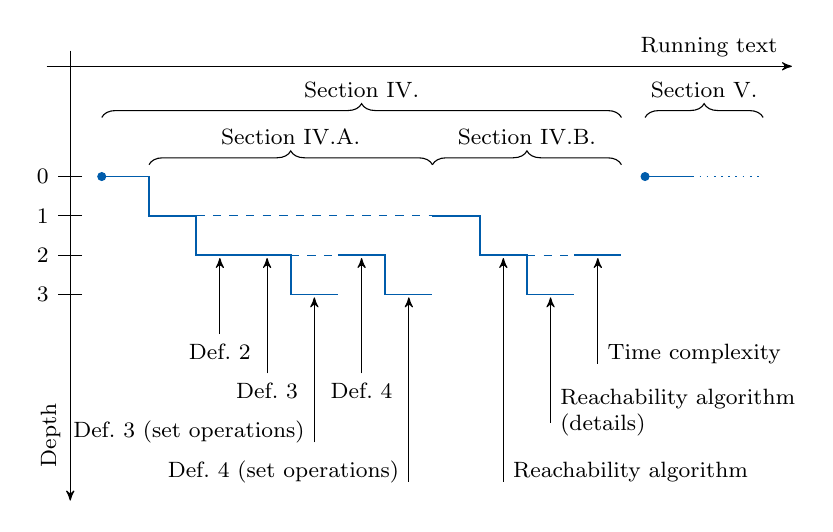
\begin{tikzpicture}[
    every node/.style={font=\footnotesize},
    stealtharrow/.style={->,>=stealth',shorten >= 1pt}
]
    % Do not exceed total width of 10
    % \draw[red] (-0.5,0.75) rectangle (9.5,-6.0);

    % intersection is at (0,0)
    \draw[stealtharrow] (-0.3,0) -- ++(9.5,0) node[pos=0.99,yshift=0.25cm,anchor=east] {Running text};
    \draw[stealtharrow] (0,0.2) -- ++(0,-5.75) node[pos=0.85,anchor=south,rotate=90] {Depth};

    \def\xoffset{0.4}
    \def\yoffset{-1.4}
    \def\dx{0.6}
    \def\dy{0.5}
    \foreach \y in { 0, 1, 2, 3 }{
        \draw[] (0.15,\yoffset - \y*\dy) -- ++(-0.3,0) node[left] {\y};
    }

    \begin{scope}[xshift=\xoffset cm,yshift=\yoffset cm]

    \filldraw[color_guideline] (0,0) circle(0.05cm);
    \draw[color_guideline,semithick]
        (0,0)           -- ++(\dx,0)    % depth 0: title + introductory sentence
        -- ++(0,-1*\dy) -- ++(\dx,0)    % depth 1: A. + introductory sentence
        -- ++(0,-1*\dy) -- ++(\dx,0)    % depth 2: support function
        -- ++(0,+0*\dy) -- ++(\dx,0)    % depth 2: polytopes
        -- ++(0,-1*\dy) -- ++(\dx,0)    % depth 3: polytopes -- set operations
           ++(0,+1*\dy) -- ++(\dx,0)    % depth 2: (constrained) zonotopes
        -- ++(0,-1*\dy) -- ++(\dx,0)    % depth 3: (constrained) zonotopes -- set operations
           ++(0,+2*\dy) -- ++(\dx,0)    % depth 1: B.
        -- ++(0,-1*\dy) -- ++(\dx,0)    % depth 2: reachability algorithm
        -- ++(0,-1*\dy) -- ++(\dx,0)    % depth 3: reachability algorithm -- steps
           ++(0,+1*\dy) -- ++(\dx,0);   % depth 2: time complexity

    \foreach \x/\y/\L in {
        2*\dx / -1*\dy / 5*\dx ,
        4*\dx / -2*\dy / 1*\dx ,
        9*\dx / -2*\dy / 1*\dx
    }{
        \draw[color_guideline,dashed] (\x,\y) -- ++(\L,0);
    }

    \draw[decorate,decoration={brace,amplitude=5pt}] (0*\dx,0.75) -- ++(11*\dx,0)
        node[midway,yshift=10pt]{Section IV.};
    \draw[decorate,decoration={brace,amplitude=5pt}] (1*\dx,0.15) -- ++(6*\dx,0)
        node[midway,yshift=10pt]{Section IV.A.};
    \draw[decorate,decoration={brace,amplitude=5pt}] (7*\dx,0.15) -- ++(4*\dx,0)
        node[midway,yshift=10pt]{Section IV.B.};

    \draw[stealtharrow] (2.5*\dx,-4*\dy) -- ++(0,2*\dy) node[pos=0,anchor=north] {Def.\ 2};
    \draw[stealtharrow] (3.5*\dx,-5*\dy) -- ++(0,3*\dy) node[pos=0,anchor=north] {Def.\ 3};
    \draw[stealtharrow] (4.5*\dx,-6.75*\dy) -- ++(0,3.75*\dy)
        node[pos=0,anchor=east,yshift=0.25*\dy cm] {Def.\ 3 (set operations)};
    \draw[stealtharrow] (5.5*\dx,-5*\dy) -- ++(0,3*\dy) node[pos=0,anchor=north] {Def.\ 4};
    \draw[stealtharrow] (6.5*\dx,-7.75*\dy) -- ++(0,4.75*\dy)
        node[pos=0,anchor=east,yshift=0.25*\dy cm] {Def.\ 4 (set operations)};

    \draw[stealtharrow] (8.5*\dx,-7.75*\dy) -- ++(0,5.75*\dy)
        node[pos=0,anchor=west,yshift=0.25*\dy cm,align=left] {Reachability algorithm};
    \draw[stealtharrow] (9.5*\dx,-6.25*\dy) -- ++(0,3.25*\dy)
        node[pos=0,anchor=west,yshift=0.25*\dy cm,align=left] {Reachability algorithm \\ (details)};
    \draw[stealtharrow] (10.5*\dx,-4.75*\dy) -- ++(0,2.75*\dy)
        node[pos=0,anchor=west,yshift=0.25*\dy cm,align=left] {Time complexity};

    % next chapter
    \filldraw[color_guideline] (11.5*\dx,0) circle(0.05cm);
    \draw[color_guideline,semithick] (11.5*\dx,0) -- ++(\dx,0);
    \draw[color_guideline,semithick,dotted] (12.5*\dx,0) -- ++(1.5*\dx,0);

    \draw[decorate,decoration={brace,amplitude=5pt}] (11.5*\dx,0.75) -- ++(1.5,0)
        node[midway,yshift=10pt]{Section V.};

    \end{scope}

\end{tikzpicture}

    \caption{Graphical representation of the example for Guideline \ref{g:universals:layers}.}
    % lower layers can be skipped, continue along the dashed line
    % allows for quickly finding necessary information if required
    % allows for reading a paper on a certain depth, e.g., skip details, focus on high-level idea
    \label{fig:layers}
\end{figure}

% non-layered:
% often shorter text because of lack of structural explanation (transition sentences and the like)
% since the structure is unclear, one must traverse the entire path to find some specific information
% heavier burden on what a reader must keep in mind when reading
% difficult to separate high-level ideas from details, since mixed together


\guideline[g:universals:introductory_sentences]
    {Use introductory sentences to outline the content of the following section or subsection.}

\goodexample[{\cite[Sec.~IV.]{Wetzlinger2023TAC}}]{
    To achieve this, we first derive closed-form expressions describing how the individual errors depend on the values of each parameter \highlightpart{in Section IV-A}.
    Next, we present our automated parameter tuning algorithm \highlightpart{in Section IV-B} and prove its convergence \highlightpart{in Section IV-C}.
    Finally, we discuss further improvements to the algorithm \highlightpart{in Section IV-D} and describe the extension to output sets \highlightpart{in Section IV-E}.
}

\noindent ...
% need to refer to *all* parts (especially if substructure is given)
% in some cases, introductory sentences are overkill


\guideline[g:universals:flow]
    {Use appropriate transitions between paragraphs.}

% good: repeat words to provide a link to the previous paragraph
% bad: unclear how next paragraph relates to previous one
\goodbadexample{
    ...
}{
    ...
}

\noindent ...


\guideline[g:universals:claims]
    {Give a reason for claims.}

\goodbadexample[{\cite[Sec.~IX.]{Wetzlinger2023TAC}}]{
    \highlightempty{} Our approach is competitive regarding the computation time, even for high-dimensional systems.
}{
    An \highlightpart{evaluation on benchmarks representing the current limits for the state-of-the-art reachability tools demonstrates} that our approach is competitive regarding the computation time, even for high-dimensional systems.
}

\goodbadexample[{\cite[Sec.~VI.B.]{Wetzlinger2025TAC}}]{
    For three compact, convex, and nonempty sets $\mathcal{S}_1, \mathcal{S}_2, \mathcal{S}_3 \subset \mathbb{R}^n$, we have
    \begin{equation*}
        \textsc{conv}(\mathcal{S}_1 \ominus \mathcal{S}_3, \mathcal{S}_2 \ominus \mathcal{S}_3) \subseteq
        \textsc{conv}(\mathcal{S}_1, \mathcal{S}_2) \ominus \mathcal{S}_3 .
    \end{equation*}
    \highlightempty{}
}{
    \textit{Lemma 1 (Distributivity of Minkowski difference over convex hull)}: For three compact, convex, and nonempty sets $\mathcal{S}_1, \mathcal{S}_2, \mathcal{S}_3 \subset \mathbb{R}^n$, we have
    \begin{equation*}
        \textsc{conv}(\mathcal{S}_1 \ominus \mathcal{S}_3, \mathcal{S}_2 \ominus \mathcal{S}_3) \subseteq
        \textsc{conv}(\mathcal{S}_1, \mathcal{S}_2) \ominus \mathcal{S}_3 .
    \end{equation*}
    \highlightpart{\textit{Proof}}: See appendix. \hfill $\square$
}

\goodbadexample[{\cite[Sec.~1]{Wetzlinger2021HSCC}}]{
    Since exact reachable sets can only be computed for a limited number of system classes \highlightempty{}, reachability algorithms compute over-approximations to establish soundness.
}{
    Since exact reachable sets can only be computed for a limited number of system classes \highlightpart{[36]}, reachability algorithms compute over-approximations to establish soundness.
}

\noindent
In scientific writing, every claim about a behavior or result should be supported by clear reasoning and never left without a solid basis.
Depending on the complexity of the statement, this justification may take the form of a brief explanation, a formal proof, or a reference to established work where the claim is substantiated.



\chapter{Introduction}
\label{ch:introduction}

Commonly, the introduction section consists of three parts:
First, it presents the research field, motivatives its importance, and narrows down to the specific research question addressed by this paper.
Next, an overview of related work contextualizes the research question by discussing related questions and approaches, while identifying the gap in current knowledge or limitations of existing methods.
Finally, it concisely outlines the paper's contributions in addressing that gap.


\guideline{Structurally separate the motivation, related work, and contributions.}

\goodbadexample{
    ...
}{
    ...
}

\noindent ...
% - type of separation depends on length of paper



\guideline[g:introduction:motivation]
    {Explain the purpose of the research field, then narrow the focus to your specific topic.}

% use first paragraph of one of the papers (inner approx)
% bad: no explain at all? or jump directly to specific topic without providing any context
\goodbadexample{
    ...
}{
    ...
}

\noindent ...
% - the first paragraph must explain the purpose of the research field, and go from broad to specific until the topic of this paper is reached



\guideline{...}
% - for broad topics, explicitly restrict the scope of the related work overview

\goodbadexample{
    ...
}{
    ...
}

\noindent ...


\guideline[g:introduction:relatedwork_structure]
    {Organize the related work into paragraphs to separate subtopics.}

\goodexample[{\cite[Sec.~1.1]{Wetzlinger2023HSCC}}]{
    \tcolorboxindent{} Since the reachable set is \highlightpart{a zero sublevel set solution of a Hamilton-Jacobi-Isaacs partial differential equation} [41], (...) \\
    \tcolorboxindent{} \highlightpart{Simulations} from a sample of initial states within the initial set can be used to construct reachable sets [19]; (...) \\
    \tcolorboxindent{} Another group of methods is \highlightpart{based on set propagation} [5].
    These methods either (...) \\
    \tcolorboxindent{} In contrast to the above algorithms for outer-approximations, \highlightpart{approaches for inner-approximations} (...) \\
    \tcolorboxindent{} For successful \highlightpart{verification}, the computed outer-approximation of the reachable set (...)
}

\noindent
Related work often divides naturally into subtopics that offer distinct perspectives on the research question.
Help readers clearly distinguish these perspectives by dedicating one paragraph to each subtopic, and let the opening phrase of the first sentence act as an implicit header---as highlighted in the above example.
If the discussion of individual subtopics becomes extensive, use subsections instead of paragraphs to maintain clarity and structure.


\guideline{...}
% - summarize related approaches in 1-2 sentences, explaining their applicability and limitations

\goodbadexample{
    ...
}{
    ...
}

\noindent ...


\guideline{Strictly separate related work and your contributions.}
% - don't mix in your contributions into the related work, use a separate paragraph for the contributions

\goodbadexample{
    ...
}{
    ...
}

\noindent ...



\guideline[g:introduction:transition_relatedwork_contributions]
    {Relate the limitations from the related work to the contributions.}

\goodexample[{\cite[Sec.~I.A.-B.]{Wetzlinger2023TAC}}]{
    \location{Related work} \\
    These tools \highlightpart{still require manual tuning} of the algorithm parameters to obtain tight approximations. (...) \\
    In conclusion, there \highlightpart{does not yet exist a fully automated parameter tuning algorithm} for linear systems that \highlightpart{satisfies an error bound} in terms of the Hausdorff distance to the exact reachable set. \par
    \location{Contributions} \\
    (...) we provide an \highlightpart{automated reachability algorithm} (Algorithm 2) that adaptively \highlightpart{tunes all the algorithm parameters} so that \highlightpart{any desired error bound} in terms of the Hausdorff distance between the exact reachable set and the computed outer approximation is respected at all times (see Section IV).
    \goodexpl{Clear link between limitations and contributions: manual vs.\ automated, no automated algorithm vs.\ automated algorithm.}
}

\noindent
Readers must clearly understand what problem the paper addresses, so the contributions should be explicitly tied to the limitations of prior work.
Each contribution should respond directly to a specific shortcoming in the state of the art, using consistent wording or even restating the limitation when appropriate.
Avoid leaving these connections implicit.



\guideline[g:introduction:contribution_bullet_points]
    {Consider presenting your contributions using bullet points.}

% each bullet point should have a strong message
% bad: merge into confusing blob paragraph
\goodbadexample{
    ...
}{
    ...
}

\noindent ...
% especially when there a multiple contributions
% if there is just a single idea (short papers), then a paragraph might be better


\guideline{Avoid mentioning methods and code releases as contributions.}

\goodbadexample{
    ...
}{
    ...
}

\noindent ...
% what is a method: "we use X to do Y"... there must be more to it than just "i did it differently"
% put "we provide code" immediately after the contributions


\guideline[g:introduction:outline_structure]
    {Outline the structure of the paper.}

\goodexample[{\cite[Sec.~1.2]{Wetzlinger2023HSCC}}]{
    We first introduce the general notation as well as set representations and operations \highlightpart{in Sec. 2} and formally define the problem statement \highlightpart{in Sec. 3}.
    Afterward, we provide a comprehensive summary of the reachability algorithm in [4] for computing outer-approximations \highlightpart{in Sec. 4.1}.
    Our contributions are as follows:
    \begin{itemize}
        \item First, we present a novel reachability algorithm using support functions to compute inner-approximations (\highlightpart{Sec. 4.2}).
        \item Next, we design a fully-automated verification algorithm for the special case of unsafe sets given as halfspaces (\highlightpart{Sec. 5.1}).
        \item Moreover, we propose a fully-automated verification algorithm for arbitrary convex unsafe sets (\highlightpart{Sec. 5.2}).
        \item In case of a safety violation, our verification algorithms return a counterexample, which provides valuable insights to system engineers (\highlightpart{Sec. 5.1-5.2}).
    \end{itemize}
    Overall, our paper provides a complete description of support function reachability, combining outer- and inner-approximation with automated verification in a self-contained presentation. 
    In contrast to previous work on reachability analysis using support functions, we provide the first approach that automatically verifies a given problem in decidable cases.
    Finally, the practical benefits of our novel algorithms are demonstrated on several challenging benchmark problems \highlightpart{in Sec. 6}.
}

\goodexample[{\cite{Wetzlinger2024ARCH2}}]{
    \highlightpart{In Section 2}, we define the halfspace representation and the vertex representation.
    Then, we introduce the object class implemented in CORA \highlightpart{in Section 3}, which also contains several set properties to improve computational efficiency.
    Afterward \highlightpart{in Section 4}, we define all implemented operations, including conversions between representations, predicates, as well as unary and binary set operations.
    Our numerical evaluation \highlightpart{in Section 5} compares our implementation with the multi-parametric toolbox [10].
}

\noindent 
As shown in the first example, one can seamlessly integrate the outline of the structure into the contributions. This is recommendable for shorter works or a more compact list of contributions.

The second example shows the more classical approach of using a separate paragraph for the outline of the paper.
This is often the last paragraph of the introduction, or even a separate subsection if the introduction has subsections.

For papers of short length (6 pages or less), it can sometimes be advisable to skip the structure outline and use that space in other parts of the paper.

\guideline[g:introduction:roadmap_empty_sentences]
    {Avoid empty sentences when outlining the structure.}

\goodbadexample{
    ...
}{
    ...
}

\noindent ...
% only relevant if the structure is a separate paragraph/section
% however, no empty sentence ("section 4 provides numerical experiments"), rather a summary of the content of each section



\chapter{Preliminaries}
\label{ch:preliminaries}

The preliminaries section clarifies the notation, fundamentals, and prior work so that readers have the necessary background to follow the main body.
Furthermore, it helps to distinguish between existing knowledge and new contributions.


\guideline{Use a separate subsection or paragraph for the notation.}

\goodbadexample{
    ...
}{
    ...
}

\noindent ...
Note: The paragraph may also be moved to the end of the introduction.


\guideline[g:preliminaries:notation_convention]
    {Ensure your notation follows standard conventions.}

% TODO: separate guideline for following wording conventions?
\goodbadexample[{\cite[Sec.~II.B.]{Wetzlinger2024CSL}}]{
    We consider autonomous nonlinear continuous-time systems
    \begin{equation*}
        \highlightpartmath{\dot{s}}(t) = \highlightpartmath{g}\big(\highlightpartmath{s}(t)\big) ,
    \end{equation*}
    where $\highlightpartmath{s} \in \mathbb{R}^n$ is the state vector and $\highlightpartmath{g}\colon \mathbb{R}^n \to \mathbb{R}^n$ is sufficiently smooth.
}{
    We consider autonomous nonlinear continuous-time systems
    \begin{equation*}
        \highlightpartmath{\dot{x}}(t) = \highlightpartmath{f}\big(\highlightpartmath{x}(t)\big) ,
    \end{equation*}
    where $\highlightpartmath{x} \in \mathbb{R}^n$ is the state vector and $\highlightpartmath{f}\colon \mathbb{R}^n \to \mathbb{R}^n$ is sufficiently smooth.
}

\noindent ...
% easier to read for the general audience if the variable have an expected meaning instead of actively translating


\guideline[g:preliminaries:lookup]
    {Use the preliminaries as a dense look up for the main body.}

\goodbadexample[{\cite[Sec.~2.1 \& Sec.~3.3]{Wetzlinger2024ARCH1}}]{
    \location{Main Body}
    Given a random direction $\ell \in \mathbb{R}^r, \left\| \ell \right\|_2 = 1$, we compute the support vector $\widehat{y}(\ell)$ associated to the support function of the computed outer approximation $\widehat{\mathcal{Y}}([0,t_{\text{end}}])$, i.e.,
    \begin{equation*}
        \widehat{y}(\ell) = \rho \big( \widehat{\mathcal{Y}}([0,t_{\text{end}}]), \ell \big) = \max_{k \in \{0,\dots,\omega - 1\}} \rho \big( \widehat{\mathcal{Y}}(\tau_k) , \ell \big) ,
    \end{equation*}
    \highlightpart{where the support function in a direction $\ell \in \mathbb{R}^n$ is defined by $\rho(\mathcal{S},\ell) \coloneqq \max_{x \in \mathcal{S}} \ell^\top x$}.
    \badexpl{The main body here also ``introduces'' known concepts, which blurs the lines between preexisting knowledge and novel contributions.}
}{
    \location{Preliminaries}
    \highlightpart{The support function in a direction $\ell \in \mathbb{R}^n$ is defined by $\rho(\mathcal{S},\ell) \coloneqq \max_{x \in \mathcal{S}} \ell^\top x$} (...).
    \location{Main Body}
    Given a random direction $\ell \in \mathbb{R}^r, \left\| \ell \right\|_2 = 1$, we compute the support vector $\widehat{y}(\ell)$ associated to the support function of the computed outer approximation $\widehat{\mathcal{Y}}([0,t_{\text{end}}])$, i.e.,
    \begin{equation*}
        \widehat{y}(\ell) = \rho \big( \widehat{\mathcal{Y}}([0,t_{\text{end}}]), \ell \big) = \max_{k \in \{0,\dots,\omega - 1\}} \rho \big( \widehat{\mathcal{Y}}(\tau_k) , \ell \big) .
    \end{equation*}
    \goodexpl{The use of support functions is now decoupled from their definition, which allows for a better focus on the actual contributions.}
}

\noindent
Ideally, preliminaries are written in a way that allows readers already familiar with the research topic or notation to skip them.
Avoid introducing essential concepts at the point of first use in the main body, especially if they are referenced multiple times throughout the paper.
Even if a concept is used only once, it is preferable to place prior knowledge in the preliminaries section for a clear separation from your contributions.


\guideline[g:preliminaries:title]
    {Consider a different section title.}

\goodexample[{\cite{Wetzlinger2024ARCH2}}]{
    ``2 Polyhedra and Polytopes''
}
% use bits of the text to justify the section title

\noindent ...
% works well if the topic of the paper is quite narrow/can be summarized well
% note: say that "preliminaries" would be bad version, but can't be truly bad, because many papers do that


\guideline[g:preliminaries:references]
    {Provide references for formulae.}

\goodbadexample[{\cite[Sec.~III.]{Wetzlinger2023TAC}}]{
    The particular solution due to the time-varying input within the set $\mathcal{U}_0$ can be enclosed by \highlightempty{}
    \begin{equation*}
        \widehat{\mathcal{P}}^\mathcal{U}(\Delta t) = \bigoplus_{i=0}^\eta \frac{A^i \Delta t^{i+1}}{(i+1)!} \, \mathcal{U}_0 \mathbf{E}(\Delta t, \eta) \Delta t \, \mathcal{U}_0 .
    \end{equation*}
}{
    The particular solution due to the time-varying input within the set $\mathcal{U}_0$ can be enclosed by \highlightpart{[12, Eq.~(3.7)]}
    \begin{equation*}
        \widehat{\mathcal{P}}^\mathcal{U}(\Delta t) = \bigoplus_{i=0}^\eta \frac{A^i \Delta t^{i+1}}{(i+1)!} \, \mathcal{U}_0 \mathbf{E}(\Delta t, \eta) \Delta t \, \mathcal{U}_0 .
    \end{equation*}
}

\noindent
Arguably, references can be forgone if the formula follows directly, e.g., by insertion, from a definition or a previous equation.
References are not necessary if the cited content is established textbook knowledge.


\guideline{...}
% - use subsections for further structuring if too long

\goodbadexample{
    ...
}{
    ...
}

\noindent ...


\guideline{Provide all information required to formulate the problem statement.}

\goodbadexample{
    ...
}{
    ...
}

\noindent ...



\chapter{Main Body}
\label{ch:mainbody}

The main body presents and analyzes the authors' approach to the research question, often divided into sections or subsections aligned with the contributions outlined in the introduction.
It is typically the longest and most technical part of the paper.


\guideline{...}
% whenever claiming something behaves in a certain way, provide a reason (or a reference)

\goodbadexample{
    ...
}{
    ...
}

\noindent ...


\guideline[g:mainbody:environments]
    {Use mathematical results and non-text elements to break the rigid structure of the running text.}

\goodbadexample{
    ...
}{
    ...
}

\noindent ...


\guideline[g:mainbody:highlevel_idea]
    {For complex derivations, begin with a separate paragraph outlining the high-level idea.}

\goodexample[{\cite[Sec.~V.B.1)]{Wetzlinger2025TAC}}]{
    Let us first \highlightpart{introduce our high-level idea} for computing an outer approximation of (43):
    Note that the intersection of any number of $\mathcal{R}_\exists(-\tau; u^*(\cdot))$ in (43) always leads to a sound outer approximation.
    Obviously, we want a tight outer approximation, that is, a small intersection stemming from a well selected, finite number of input trajectories $u^*(\cdot) \in \mathbb{U}$.
    For this selection, we use a heuristic approach via support function reachability, which simplifies the intersection of the individual reachable sets in (43).
}

\noindent ...
% use case: multiple paragraphs/steps to result


\guideline[g:mainbody:introductory_sentences]
    {Use introductory sentences to outline the content of the following section.}

% EASY
% find a good one
\goodexample{
    ...
}

\noindent ...
% in some cases, introductory sentences are overkill


\guideline[g:mainbody:proofs_appendix]
    {Consider moving proofs to an appendix.}

\goodexample[{\cite[Proposition 3 \& Appendix]{Wetzlinger2025TAC}}]{
    \textit{Proposition 3 (Time-point AE backward reachable set)}:
    The backward reachable set $\mathcal{R}_{\forall\exists}(-t)$ defined in (32) can be computed by
    \begin{equation*}
        \mathcal{R}_{\forall\exists}(-t) = e^{-At} \big( (\mathcal{X}_{\text{end}} \oplus \mathcal{Z}_{\mathcal{}W}(t)) \ominus \mathcal{Z}_{\mathcal{U}}(t) \big) .
    \end{equation*}
    \highlightpart{\textit{Proof:} See Appendix.}
    \\
    (...)
    \highlightpart{\textit{Proof of Proposition 3:}} We have
    \begin{align*}
        &x_0 \in e^{-At} \big( (\mathcal{X}_{\text{end}} \oplus -\mathcal{Z}_{\mathcal{W}}(t) ) \ominus \mathcal{Z}_{\mathcal{U}}(t) \big) \\
        &\Leftrightarrow \forall z_u \in \mathcal{Z}_\mathcal{U}(t)\colon e^{At} x_0 + z_u \in \mathcal{X}_{\text{end}} \ominus -\mathcal{Z}_{\mathcal{W}}(t) \\
        &\Leftrightarrow \forall z_u \in \mathcal{Z}_\mathcal{U}(t) \exists z_w \in \mathcal{Z}_{\mathcal{W}}(t) \colon e^{At} x_0 + z_u + z_w \in \mathcal{X}_{\text{end}} \\
        &\Leftrightarrow \forall u(\cdot) \in \mathbb{U} \exists w(\cdot) \in \mathbb{W}\colon \xi(t; x_0, u(\cdot), w(\cdot)) \in \mathcal{X}_{\text{end}}
    \end{align*}
    which is equal to the definition in (32). \hfill $\square$
}

\noindent
Moving proofs to an appendix helps maintain the focus on the statement and its relation to the surrounding content.
In particular, technical proofs require a lot of attention from the reader, and such a deep dive may lead to losing sight of the bigger picture.
Still, if the proofs are few and simple, it is preferable to keep them in the main body.
Avoid keeping some in the main body and moving others to the appendix---make it an all-or-nothing decision.


\guideline{...}
% consider a running example if the contributions allow for that and the notation is difficult to understand, but fairly easy once you do understand it

\goodbadexample{
    ...
}{
    ...
}

\noindent ...


\guideline[g:mainbody:subsections]
    {Organize contributions into multiple sections.}

\goodbadexample{
    ...
}{
    ...
}

\noindent ...
% - use multiple sections for distinct approaches (e.g., linear, then nonlinear)


\guideline{Use appropriate transitions between paragraphs.}

\goodbadexample{
    ...
}{
    ...
}

\noindent ...



\chapter{Results}
\label{ch:results}

The numerical evaluation quantitatively measures the performance of the proposed approach, typically comparing it to state-of-the-art methods across several metrics, particularly computation time and accuracy. The selected examples should span a variety of application scenarios to robustly support the claims made in the main body.


\guideline[g:results:motivate_examples]
    {Motivate the selection of examples.}

\goodbadexample[{\cite[Sec.~VII.A.-C.]{Wetzlinger2023TAC}}]{
    \location{Sec.VII.A.} \\
    \highlightpart{We first consider the deliberately simple example} (...) \\
    \location{Sec.VII.B.} \\
    Next, we evaluate our verification algorithm on \highlightpart{benchmarks from the 2021 ARCH competition [53]}, which are (...) \\
    \location{Sec.VII.C.} \\
    Finally, we \highlightpart{evaluate our verification algorithm on the benchmark proposed in [54]}, where (...)
}{
    \location{Sec.VII.A.} \\
    To \highlightpart{showcase the general concept of our approach}, we first consider the deliberately simple example (...) \\
    \location{Sec.VII.B.} \\
    Next, we evaluate our verification algorithm on \highlightpart{benchmarks from the 2021 ARCH competition [53], where state-of-the-art reachability tools compete with one another to solve challenging verification tasks. We consider all linear continuous-time systems}, which are (...) \\
    \location{Sec.VII.C.} \\
    Finally, we show that our verification algorithm can \highlightpart{handle complex verification tasks featuring time-varying specifications. To this end, we consider} the benchmark proposed in [54], where (...)
}

\noindent
Explain why each example was chosen.
For instance, you might use a simple example to illustrate a core concept, a larger one to demonstrate scalability, or a challenging benchmark for comparison with the state of the art.
Avoid merely listing examples or their sources without clarifying their purpose or relevance.


\guideline[g:results:specs]
    {List the system specifications of the machine used to run the evaluation.}

\goodbadexample{
    ...
}{
    ...
}

\noindent ...


\guideline[g:results:same_machine]
    {If possible, run all evaluations on the same machine.}

\goodexample[{\cite[Sec.~5]{Wetzlinger2024ARCH2}}]{
    Additionally, we provide a \highlightpart{comparison to the multi-parametric toolbox} in terms of the computation times for an increasing dimension.
    \highlightpart{All computations} are carried out on an AMD Ryzen 5 5600H processor with a 3.30 GHz Radeon Graphics unit and 16GB memory.
}

\noindent
If timing is relevant, running all evaluations on the same machine ensures a level playing field for comparison between approaches.
System specifications can significantly impact the timings, so keeping them consistent helps isolate differences in performance.
Of course, this may not be possible if the code for certain approaches is not available.


\guideline{...}
% - one subsection per group of examples
% - subsections should be roughly of equal length

\goodbadexample{
    ...
}{
    ...
}

\noindent ...


\guideline{Compare your approach to approaches from the literature.}

\goodbadexample{
    ...
}{
    ...
}

\noindent ...
% if new research question addressed, use a simpler example where there is common ground


\guideline[g:results:data]
    {Provide all data required for running the numerical experiments.}

% find an example that is short enough but extensive enough at the same time
\goodexample{
    ...
}

\noindent ...
% either directly (vectors, matrices, ...) or as repeatability package


\guideline[g:results:tables]
    {Use tables to present metrics.}

\goodbadexample[{\cite[Sec.~VII.A \& Tab.~II]{Wetzlinger2025TAC}}]{
    While the runtime complexity of our proposed algorithms only scales linearly with the number of time steps, the computation time of HJ reachability strongly depends on the partitioning on the grid, as it suffers from the curse of dimensionality.
    \highlightpart{Using $n_{\text{grid}} = 15$ grid points per dimension results in a computation time of $2.4\si{\second}$ in both cases, and $n_{\text{grid}} = 35$ already about $200\si{\second}$.}
}{
    While the runtime complexity of our proposed algorithms only scales linearly with the number of time steps, the computation time of HJ reachability strongly depends on the partitioning on the grid, \highlightpart{see Table II}, as it suffers from the curse of dimensionality.

    \begin{center}
\begin{small}
Table II: Results of Sections VII-A to VII-C.
\end{small}

\smallskip

\begin{footnotesize}
\begin{tabular}{l l l}
	\toprule
	\textbf{Benchmark} & \textbf{Algorithm} & \textbf{Time} \\ \midrule
	\multirow{3}{*}{Section VII-A: $\widehat{\mathcal{R}}_{\forall\exists}(-\tau)$} & Alg.\ 2 ($\sigma = 100$) & $0.11\si{\second}$ \\
	& \highlightpart{HJ ($n_{\text{grid}} = 15$)} & \highlightpart{$2.4\si{\second}$} \\
	& \highlightpart{HJ ($n_{\text{grid}} = 35$)} & \highlightpart{$197\si{\second}$} \\ \midrule
	\multirow{3}{*}{Section VII-A: $\widecheck{\mathcal{R}}_{\exists\forall}(-\tau)$} & Alg.\ 3 ($\sigma = 100$) & $0.12\si{\second}$ \\
	& \highlightpart{HJ ($n_{\text{grid}} = 15$)} & \highlightpart{$2.4\si{\second}$} \\
	& \highlightpart{HJ ($n_{\text{grid}} = 35$)} & \highlightpart{$194\si{\second}$} \\ \midrule
	$\cdots$ & & \\
	\bottomrule
\end{tabular}
\end{footnotesize}
\end{center}
}

\noindent
Tables present data in a compact and well-structured format, allowing readers to easily compare results at a glance.
Use tables to display raw values, while reserving the running text for interpretations and explanations.


\guideline[g:results:explain_results]
    {Explain and interpret the results.}

\badexample[{\cite[Sec.~V.]{Wetzlinger2024CSL}}]{
    Algorithm 1 is faster than the scaling approach [10] by orders of magnitude and even faster than the C++ implementation of the projection approach [5].
    \highlightempty{}
}

\newpage

\goodexample{
    Algorithm 1 is faster than the scaling approach [10] by orders of magnitude and even faster than the C++ implementation of the projection approach [5]. (...)
    \highlightpart{Most computation time is spent on the range bounding in (9) using interval arithmetic, which explains the fast evaluation of the Lotka-Volterra and Biological Model benchmarks whose Hessian tensor is constant.}
}

\noindent
While the raw data of the numerical evaluation is best presented in a table, it is still good practice to briefly summarize the results in the running text.
Furthermore, provide an explanation for general trends by linking to the properties of the respective approaches.
Also, explain surprising findings---often, these cases exhibit a particular exploitable structure.



\chapter{Discussion and Conclusion}
\label{ch:conclusion}

The conclusion ties together the research question, the present approach, and the results.
Briefly discussing the limitations helps identify potential directions for future work.


\guideline[g:conclusion:discussion_section]
    {Discuss your work in a broader frame of reference.}

% make the comparison to the literature that was not possible before the main body
\goodexample{
    ...
}

\noindent ...
% only make a separate discussion section if necessary (probably not for shorter papers)


\guideline[g:conclusion:summary]
    {Briefly summarize the contributions and the results.}

\goodbadexample{
    ...
}{
    ...
}

\noindent ...


\newpage


\guideline{Avoid repeating the abstract.}

\goodbadexample{
    ...
}{
    ...
}

\noindent ...


\newpage


\guideline[g:conclusion:limitations]
    {Address limitations of your work.}

% bad would be to not mention anything
\goodexample{
    ...
}

\noindent ...
% - point out large enough weaknesses/next steps, the audience does not expect them to be solved in this paper due to space restrictions (smaller things are difficult to argue: why not done here?)


\guideline[g:conclusion:future_work]
    {Give directions for future work.}

\goodexample[{\cite[Sec.~VI.]{Wetzlinger2024CSL}}]{
    Future work will address nonautonomous nonlinear systems, where the main challenge is to design a reachability algorithm that can efficiently evaluate both the Minkowski difference and the Minkowski sum.
}

\noindent ...
% may contain ideas/directions for future work (non-trivial extensions, different applications, ...)
% also mention challenges that may come up (see example)




% %%%% LOW LEVEL %%%%
\part{Writing and Formatting}


\chapter{Figures, Tables, and Pseudocode}
\label{ch:nontextelements}

Non-text elements such as figures, tables, and pseudocode play a crucial role in organizing the flow of the work.
By effectively using these components---in \LaTeX{}, via the use of so-called environments---, authors ensure an effective communication of their content.

% general

\guideline[g:nontext:refer_non_text_elements]
    {Refer to all non-text elements in the running text.}

\goodbadexample{
    ...
}{
    ...
}

\noindent The placement of non-text elements like figures, tables, and algorithms with respect to the running text is typically managed by \LaTeX{}, so readers often skip over them until a reference directs them to a specific element.
Therefore, it is good practice to explicitly reference each non-text element, ideally in a separate paragraph explaining its content.
% An alternative formulation to this guideline is:
% ``Only use environments if they are referenced at least once later.''


\guideline[g:nontext:placement_top]
    {Place non-text elements on the top of a page or column.}

\goodbadexample[{\cite[Sec.~II.B.]{Wetzlinger2025TAC}}]{
    \location{Top of the page} \\
    (...) \\
    The exact conversion from a polytope to a constrained zonotopes, denoted by $\textsc{CZ}(\mathcal{P})$, is computed using Algorithm 1, which implements [12, Thm. 1].
    
    \algruletop{}
\textbf{Algorithm 1} ~ Conversion: Polytope to constrained zonotope. \\
\textbf{Input:} Polytope $\mathcal{P} = \langle H, d \rangle_P$ \\
\textbf{Output:} Constrained zonotope $\mathcal{CZ} = \langle c, G, K, l \rangle_{CZ}$

\begin{algorithmic}[1]
	\State $\langle c, G \rangle_Z \gets \textsc{box}( \mathcal{P} )$
    \State $\forall j \in \mathbb{N}_{[1,...,h]}\colon o_{(j)} \gets -\rho\big( \langle c, G \rangle_Z,-H_{(j,\cdot)}^\top \big)$
    \State $G \gets [G \;\, \mathbf{0}]$, $K \gets [H G \;\, \tfrac{1}{2}\mathrm{diag}(o - d)]$, $l \gets \tfrac{1}{2}(d+o) - Hc$
    \State $\mathcal{CZ} \gets \langle c, G, K, l \rangle_{CZ}$
\end{algorithmic}
\algrulebottom{}


    The convex hull can be computed according to [13, Thm. 5] and the multiplication with an intervalmatrix $\mathbf{M}\mathcal{CZ}$ follows from (16).
}{
    \location{Top of the page} \\
    \algruletop{}
\textbf{Algorithm 1} ~ Conversion: Polytope to constrained zonotope. \\
\textbf{Input:} Polytope $\mathcal{P} = \langle H, d \rangle_P$ \\
\textbf{Output:} Constrained zonotope $\mathcal{CZ} = \langle c, G, K, l \rangle_{CZ}$

\begin{algorithmic}[1]
	\State $\langle c, G \rangle_Z \gets \textsc{box}( \mathcal{P} )$
    \State $\forall j \in \mathbb{N}_{[1,...,h]}\colon o_{(j)} \gets -\rho\big( \langle c, G \rangle_Z,-H_{(j,\cdot)}^\top \big)$
    \State $G \gets [G \;\, \mathbf{0}]$, $K \gets [H G \;\, \tfrac{1}{2}\mathrm{diag}(o - d)]$, $l \gets \tfrac{1}{2}(d+o) - Hc$
    \State $\mathcal{CZ} \gets \langle c, G, K, l \rangle_{CZ}$
\end{algorithmic}
\algrulebottom{}

    
    (...) \\
    The exact conversion from a polytope to a constrained zonotopes, denoted by $\textsc{CZ}(\mathcal{P})$, is computed using Algorithm 1, which implements [12, Thm. 1].
    The convex hull can be computed according to [13, Thm. 5] and the multiplication with an intervalmatrix $\mathbf{M}\mathcal{CZ}$ follows from (16).
}

\noindent Placing non-text elements at the top of the page or column offers several advantages:
First, these elements are easily accessible when referenced in the text.
Second, non-text elements often condense important information, warranting prominent placement, such as at the top of the page.
Third, this placement preserves the flow of the running text, contributing to optimizing space usage.

% figures

\guideline[g:nontext:figure_vector_graphics]
    {Figures: Use vector graphics.}

% bad: make bad screenshot of vector graphics
\goodbadexample{
    ...
}{
    ...
}

\noindent No exceptions.
Since figures typically capture the reader's attention first, investing in high-quality figures is well worth the effort.
Many applications offer the ability to export a drawn canvas as a vector graphics file.



\guideline[g:nontext:figure_same_font]
    {Figures: Use the same font and font sizes as in the running text.}

% bad: different font due to image generating program (or image screenshot, etc.)
\goodbadexample{
    ...
}{
    ...
}

\noindent Using the same font and font sizes in figures as in the running text allows the figure to blend seamlessly with the rest of the document, contributing to a cohesive overall appearance.
This is most easily achieved with the \LaTeX{} package \emph{TikZ}, as it compiles the text in figures using the same settings as the rest of the document.


\guideline[g:nontext:figure_colorvisiondeficiency]
    {Figures: Ensure colors are distinguishable.}

\goodbadexample[{\cite[Fig.~3]{Wetzlinger2023HSCC}}]{
    % This file was created by matlab2tikz.
%
%The latest updates can be retrieved from
%  http://www.mathworks.com/matlabcentral/fileexchange/22022-matlab2tikz-matlab2tikz
%where you can also make suggestions and rate matlab2tikz.
%
\definecolor{mycolor1}{rgb}{0.00000,0.36078,0.67059}%
\definecolor{mycolor2}{rgb}{0.89020,0.10588,0.13725}%

\tikzsetnextfilename{figure_cvd_bad}
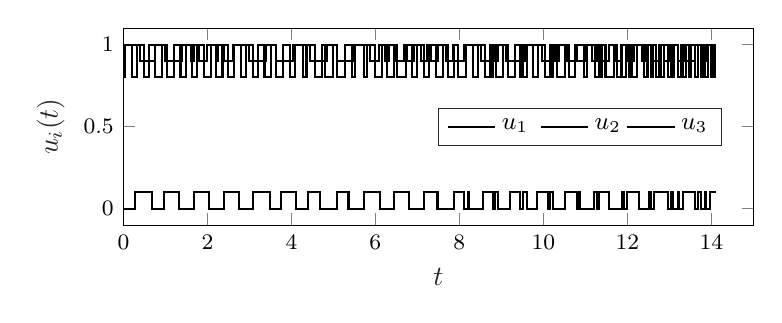
\begin{tikzpicture}

\begin{axis}[%
width=8cm,
height=2.5cm,
at={(0in,0in)},
scale only axis,
xmin=0.000,
xmax=15.000,
xlabel style={font=\color{white!15!black}},
xlabel={$t$},
ymin=-0.100,
ymax=1.100,
ylabel style={font=\color{white!15!black}},
ylabel={$u_i(t)$},
axis background/.style={fill=white},
legend columns = 3,
legend style={legend cell align=left, font=\small, align=left, draw=white!15!black,
	at={(0.95,0.5)}, anchor=east,
	/tikz/column 2/.style={column sep=0.075cm}},
%legend image post style={line width = 1pt},
every tick label/.append style={font=\footnotesize}
]

\addplot [color=black, line width=0.75pt]
  table[row sep=crcr]{%
0.000	0.000\\
0.280	0.000\\
0.280	0.100\\
0.680	0.100\\
0.680	0.000\\
0.960	0.000\\
0.960	0.100\\
1.320	0.100\\
1.320	0.000\\
1.680	0.000\\
1.680	0.100\\
2.040	0.100\\
2.040	0.000\\
2.400	0.000\\
2.400	0.100\\
2.760	0.100\\
2.760	0.000\\
3.080	0.000\\
3.080	0.100\\
3.480	0.100\\
3.480	0.000\\
3.760	0.000\\
3.760	0.100\\
4.120	0.100\\
4.120	0.000\\
4.400	0.000\\
4.400	0.100\\
4.680	0.100\\
4.680	0.000\\
5.080	0.000\\
5.080	0.100\\
5.360	0.100\\
5.360	0.000\\
5.720	0.000\\
5.720	0.100\\
6.120	0.100\\
6.120	0.000\\
6.440	0.000\\
6.440	0.100\\
6.800	0.100\\
6.800	0.000\\
7.160	0.000\\
7.160	0.100\\
7.480	0.100\\
7.480	0.000\\
7.880	0.000\\
7.880	0.100\\
8.120	0.100\\
8.120	0.000\\
8.200	0.000\\
8.200	0.100\\
8.240	0.100\\
8.240	0.000\\
8.560	0.000\\
8.560	0.100\\
8.800	0.100\\
8.800	0.000\\
8.840	0.000\\
8.840	0.100\\
8.920	0.100\\
8.920	0.000\\
9.200	0.000\\
9.200	0.100\\
9.440	0.100\\
9.440	0.000\\
9.520	0.000\\
9.520	0.100\\
9.600	0.100\\
9.600	0.000\\
9.840	0.000\\
9.840	0.100\\
10.120	0.100\\
10.120	0.000\\
10.160	0.000\\
10.160	0.100\\
10.240	0.100\\
10.240	0.000\\
10.520	0.000\\
10.520	0.100\\
10.800	0.100\\
10.800	0.000\\
10.840	0.000\\
10.840	0.100\\
10.880	0.100\\
10.880	0.000\\
11.200	0.000\\
11.200	0.100\\
11.280	0.100\\
11.280	0.000\\
11.320	0.000\\
11.320	0.100\\
11.560	0.100\\
11.560	0.000\\
11.880	0.000\\
11.880	0.100\\
11.920	0.100\\
11.920	0.000\\
12.000	0.000\\
12.000	0.100\\
12.280	0.100\\
12.280	0.000\\
12.520	0.000\\
12.520	0.100\\
12.560	0.100\\
12.560	0.000\\
12.640	0.000\\
12.640	0.100\\
12.960	0.100\\
12.960	0.000\\
13.040	0.000\\
13.040	0.100\\
13.080	0.100\\
13.080	0.000\\
13.200	0.000\\
13.200	0.100\\
13.240	0.100\\
13.240	0.000\\
13.320	0.000\\
13.320	0.100\\
13.600	0.100\\
13.600	0.000\\
13.680	0.000\\
13.680	0.100\\
13.760	0.100\\
13.760	0.000\\
13.840	0.000\\
13.840	0.100\\
13.880	0.100\\
13.880	0.000\\
13.960	0.000\\
13.960	0.100\\
14.120	0.100\\
};
\addlegendentry{$u_1$}

\addplot [color=black, line width=0.75pt]
  table[row sep=crcr]{%
0.000	0.800\\
0.040	0.800\\
0.040	1.000\\
0.200	1.000\\
0.200	0.800\\
0.320	0.800\\
0.320	1.000\\
0.480	1.000\\
0.480	0.800\\
0.600	0.800\\
0.600	1.000\\
0.760	1.000\\
0.760	0.800\\
0.920	0.800\\
0.920	1.000\\
1.040	1.000\\
1.040	0.800\\
1.200	0.800\\
1.200	1.000\\
1.360	1.000\\
1.360	0.800\\
1.480	0.800\\
1.480	1.000\\
1.640	1.000\\
1.640	0.800\\
1.760	0.800\\
1.760	1.000\\
1.920	1.000\\
1.920	0.800\\
2.080	0.800\\
2.080	1.000\\
2.200	1.000\\
2.200	0.800\\
2.360	0.800\\
2.360	1.000\\
2.480	1.000\\
2.480	0.800\\
2.640	0.800\\
2.640	1.000\\
2.800	1.000\\
2.800	0.800\\
2.920	0.800\\
2.920	1.000\\
3.080	1.000\\
3.080	0.800\\
3.200	0.800\\
3.200	1.000\\
3.360	1.000\\
3.360	0.800\\
3.520	0.800\\
3.520	1.000\\
3.640	1.000\\
3.640	0.800\\
3.800	0.800\\
3.800	1.000\\
3.960	1.000\\
3.960	0.800\\
4.080	0.800\\
4.080	1.000\\
4.280	1.000\\
4.280	0.800\\
4.360	0.800\\
4.360	1.000\\
4.560	1.000\\
4.560	0.800\\
4.720	0.800\\
4.720	1.000\\
4.800	1.000\\
4.800	0.800\\
5.000	0.800\\
5.000	1.000\\
5.080	1.000\\
5.080	0.800\\
5.280	0.800\\
5.280	1.000\\
5.440	1.000\\
5.440	0.800\\
5.520	0.800\\
5.520	1.000\\
5.720	1.000\\
5.720	0.800\\
5.800	0.800\\
5.800	1.000\\
6.000	1.000\\
6.000	0.800\\
6.160	0.800\\
6.160	1.000\\
6.280	1.000\\
6.280	0.800\\
6.440	0.800\\
6.440	1.000\\
6.520	1.000\\
6.520	0.800\\
6.720	0.800\\
6.720	1.000\\
6.880	1.000\\
6.880	0.800\\
7.000	0.800\\
7.000	1.000\\
7.160	1.000\\
7.160	0.800\\
7.280	0.800\\
7.280	1.000\\
7.440	1.000\\
7.440	0.800\\
7.600	0.800\\
7.600	1.000\\
7.720	1.000\\
7.720	0.800\\
7.880	0.800\\
7.880	1.000\\
7.960	1.000\\
7.960	0.800\\
8.160	0.800\\
8.160	1.000\\
8.320	1.000\\
8.320	0.800\\
8.440	0.800\\
8.440	1.000\\
8.600	1.000\\
8.600	0.800\\
8.720	0.800\\
8.720	1.000\\
8.760	1.000\\
8.760	0.800\\
8.800	0.800\\
8.800	1.000\\
8.880	1.000\\
8.880	0.800\\
9.040	0.800\\
9.040	1.000\\
9.160	1.000\\
9.160	0.800\\
9.320	0.800\\
9.320	1.000\\
9.440	1.000\\
9.440	0.800\\
9.480	0.800\\
9.480	1.000\\
9.520	1.000\\
9.520	0.800\\
9.600	0.800\\
9.600	1.000\\
9.760	1.000\\
9.760	0.800\\
9.880	0.800\\
9.880	1.000\\
10.040	1.000\\
10.040	0.800\\
10.160	0.800\\
10.160	1.000\\
10.200	1.000\\
10.200	0.800\\
10.240	0.800\\
10.240	1.000\\
10.320	1.000\\
10.320	0.800\\
10.520	0.800\\
10.520	1.000\\
10.600	1.000\\
10.600	0.800\\
10.760	0.800\\
10.760	1.000\\
10.960	1.000\\
10.960	0.800\\
11.040	0.800\\
11.040	1.000\\
11.240	1.000\\
11.240	0.800\\
11.320	0.800\\
11.320	1.000\\
11.360	1.000\\
11.360	0.800\\
11.400	0.800\\
11.400	1.000\\
11.480	1.000\\
11.480	0.800\\
11.680	0.800\\
11.680	1.000\\
11.760	1.000\\
11.760	0.800\\
11.840	0.800\\
11.840	1.000\\
11.880	1.000\\
11.880	0.800\\
11.960	0.800\\
11.960	1.000\\
12.040	1.000\\
12.040	0.800\\
12.080	0.800\\
12.080	1.000\\
12.120	1.000\\
12.120	0.800\\
12.240	0.800\\
12.240	1.000\\
12.400	1.000\\
12.400	0.800\\
12.480	0.800\\
12.480	1.000\\
12.560	1.000\\
12.560	0.800\\
12.600	0.800\\
12.600	1.000\\
12.680	1.000\\
12.680	0.800\\
12.760	0.800\\
12.760	1.000\\
12.800	1.000\\
12.800	0.800\\
12.880	0.800\\
12.880	1.000\\
12.960	1.000\\
12.960	0.800\\
13.040	0.800\\
13.040	1.000\\
13.080	1.000\\
13.080	0.800\\
13.120	0.800\\
13.120	1.000\\
13.200	1.000\\
13.200	0.800\\
13.280	0.800\\
13.280	1.000\\
13.320	1.000\\
13.320	0.800\\
13.400	0.800\\
13.400	1.000\\
13.480	1.000\\
13.480	0.800\\
13.520	0.800\\
13.520	1.000\\
13.600	1.000\\
13.600	0.800\\
13.680	0.800\\
13.680	1.000\\
13.760	1.000\\
13.760	0.800\\
13.800	0.800\\
13.800	1.000\\
13.840	1.000\\
13.840	0.800\\
13.920	0.800\\
13.920	1.000\\
14.000	1.000\\
14.000	0.800\\
14.040	0.800\\
14.040	1.000\\
14.080	1.000\\
14.080	0.800\\
14.120	0.800\\
};
\addlegendentry{$u_2$}

\addplot [color=black, line width=0.75pt]
  table[row sep=crcr]{%
0.000	1.000\\
0.400	1.000\\
0.400	0.900\\
0.760	0.900\\
0.760	1.000\\
1.000	1.000\\
1.000	0.900\\
1.400	0.900\\
1.400	1.000\\
1.600	1.000\\
1.600	0.900\\
1.680	0.900\\
1.680	1.000\\
1.800	1.000\\
1.800	0.900\\
2.000	0.900\\
2.000	1.000\\
2.200	1.000\\
2.200	0.900\\
2.240	0.900\\
2.240	1.000\\
2.400	1.000\\
2.400	0.900\\
2.600	0.900\\
2.600	1.000\\
3.000	1.000\\
3.000	0.900\\
3.400	0.900\\
3.400	1.000\\
3.640	1.000\\
3.640	0.900\\
4.040	0.900\\
4.040	1.000\\
4.440	1.000\\
4.440	0.900\\
4.840	0.900\\
4.840	1.000\\
5.080	1.000\\
5.080	0.900\\
5.480	0.900\\
5.480	1.000\\
5.880	1.000\\
5.880	0.900\\
6.080	0.900\\
6.080	1.000\\
6.240	1.000\\
6.240	0.900\\
6.320	0.900\\
6.320	1.000\\
6.480	1.000\\
6.480	0.900\\
6.680	0.900\\
6.680	1.000\\
6.760	1.000\\
6.760	0.900\\
6.920	0.900\\
6.920	1.000\\
7.080	1.000\\
7.080	0.900\\
7.240	0.900\\
7.240	1.000\\
7.320	1.000\\
7.320	0.900\\
7.480	0.900\\
7.480	1.000\\
7.680	1.000\\
7.680	0.900\\
7.840	0.900\\
7.840	1.000\\
7.880	1.000\\
7.880	0.900\\
8.120	0.900\\
8.120	1.000\\
8.520	1.000\\
8.520	0.900\\
8.760	0.900\\
8.760	1.000\\
8.840	1.000\\
8.840	0.900\\
8.920	0.900\\
8.920	1.000\\
9.120	1.000\\
9.120	0.900\\
9.560	0.900\\
9.560	1.000\\
9.960	1.000\\
9.960	0.900\\
10.160	0.900\\
10.160	1.000\\
10.280	1.000\\
10.280	0.900\\
10.360	0.900\\
10.360	1.000\\
10.560	1.000\\
10.560	0.900\\
10.760	0.900\\
10.760	1.000\\
10.800	1.000\\
10.800	0.900\\
11.000	0.900\\
11.000	1.000\\
11.160	1.000\\
11.160	0.900\\
11.280	0.900\\
11.280	1.000\\
11.400	1.000\\
11.400	0.900\\
11.560	0.900\\
11.560	1.000\\
11.720	1.000\\
11.720	0.900\\
11.880	0.900\\
11.880	1.000\\
12.000	1.000\\
12.000	0.900\\
12.160	0.900\\
12.160	1.000\\
12.360	1.000\\
12.360	0.900\\
12.440	0.900\\
12.440	1.000\\
12.600	1.000\\
12.600	0.900\\
12.800	0.900\\
12.800	1.000\\
12.880	1.000\\
12.880	0.900\\
13.000	0.900\\
13.000	1.000\\
13.200	1.000\\
13.200	0.900\\
13.360	0.900\\
13.360	1.000\\
13.400	1.000\\
13.400	0.900\\
13.600	0.900\\
13.600	1.000\\
13.840	1.000\\
13.840	0.900\\
13.880	0.900\\
13.880	1.000\\
14.000	1.000\\
14.000	0.900\\
14.120	0.900\\
};
\addlegendentry{$u_3$}

\end{axis}

\end{tikzpicture}

    \badexpl{We use only black lines to simulate how indistinguishable colors can appear to individuals with color vision deficiency.}
}{
    \input{data/figure_cvd_good.tikz}
}

\noindent
Color vision deficiency affects approximately $8\%$ of men and $0.5\%$ of women worldwide, or roughly $1$ in $12$ men and $1$ in $200$ women \footfullcite{Gordon1998}.
As a result, it is highly likely that some readers would benefit from color choices that accommodate this condition.


\guideline[g:nontext:figure_linestyles]
    {Figures: Consider using different line styles.}

\goodbadexample[{\cite[Fig.~3]{Wetzlinger2024CSL}}]{
    \input{data/figure_linestyle_bad.tikz}
}{
    % This file was created by matlab2tikz.
%
%The latest updates can be retrieved from
%  http://www.mathworks.com/matlabcentral/fileexchange/22022-matlab2tikz-matlab2tikz
%where you can also make suggestions and rate matlab2tikz.
%
\definecolor{mycolor1}{rgb}{0.00000,0.36078,0.67059}%
\definecolor{mycolor2}{rgb}{0.89020,0.10588,0.13725}%
%
\tikzsetnextfilename{figure_cvd_good}
\begin{tikzpicture}

\begin{axis}[%
width=7.5cm,
height=3.1cm,
at={(0in,0in)},
scale only axis,
xmin=0.000,
xmax=3.000,
xlabel style={font=\color{white!15!black}},
xlabel={$t$},
ymin=0.000,
ymax=1.000,
ylabel style={font=\color{white!15!black}},
ylabel={$\gamma_{\min}(t)$},
axis background/.style={fill=white},
legend columns = 3,
legend style={legend cell align=left, font=\small, align=left, draw=white!15!black,
	at={(-0.1,-0.4)}, anchor=north west,
	/tikz/column 2/.style={column sep=0.075cm}},
%legend image post style={line width = 1pt},
every tick label/.append style={font=\footnotesize}
]

\addplot [color=mycolor1, line width=1pt]
  table[row sep=crcr]{%
0	1\\
0.01	0.995\\
0.02	0.991\\
0.05	0.976\\
0.06	0.972\\
0.08	0.962\\
0.09	0.958\\
0.11	0.948\\
0.12	0.944\\
0.14	0.934\\
0.15	0.93\\
0.16	0.925\\
0.17	0.921\\
0.18	0.916\\
0.2	0.908\\
0.21	0.903\\
0.29	0.871\\
0.3	0.868\\
0.31	0.864\\
0.33	0.858\\
0.34	0.854\\
0.38	0.842\\
0.39	0.84\\
0.4	0.837\\
0.41	0.835\\
0.42	0.832\\
0.47	0.822\\
0.48	0.821\\
0.49	0.819\\
0.53	0.815\\
0.54	0.815\\
0.55	0.814\\
0.56	0.814\\
0.58	0.812\\
0.59	0.812\\
0.61	0.81\\
0.62	0.81\\
0.63	0.809\\
0.65	0.809\\
0.66	0.808\\
0.69	0.808\\
0.75	0.796\\
0.76	0.795\\
0.77	0.793\\
0.78	0.792\\
0.8	0.788\\
0.81	0.787\\
0.82	0.785\\
0.83	0.784\\
0.84	0.782\\
0.86	0.78\\
0.87	0.778\\
0.88	0.777\\
0.89	0.775\\
0.91	0.773\\
0.92	0.771\\
0.96	0.767\\
0.97	0.765\\
1.04	0.758\\
1.05	0.758\\
1.08	0.755\\
1.09	0.755\\
1.13	0.751\\
1.14	0.751\\
1.17	0.748\\
1.18	0.748\\
1.21	0.745\\
1.22	0.745\\
1.23	0.744\\
1.24	0.744\\
1.25	0.743\\
1.26	0.743\\
1.27	0.742\\
1.28	0.742\\
1.29	0.741\\
1.3	0.741\\
1.31	0.74\\
1.32	0.74\\
1.33	0.739\\
1.34	0.739\\
1.35	0.738\\
1.36	0.738\\
1.37	0.737\\
1.39	0.737\\
1.4	0.736\\
1.42	0.736\\
1.43	0.735\\
1.45	0.735\\
1.46	0.734\\
1.49	0.734\\
1.5	0.733\\
1.56	0.733\\
1.57	0.732\\
1.6	0.732\\
1.61	0.731\\
1.62	0.731\\
1.63	0.73\\
1.64	0.73\\
1.67	0.727\\
1.68	0.727\\
1.7	0.725\\
1.71	0.725\\
1.72	0.724\\
1.73	0.724\\
1.74	0.723\\
1.76	0.723\\
1.78	0.711\\
1.79	0.704\\
1.8	0.704\\
1.81	0.703\\
1.82	0.697\\
1.86	0.669\\
1.87	0.661\\
1.88	0.64\\
1.89	0.614\\
1.91	0.564\\
1.92	0.548\\
1.93	0.571\\
1.94	0.591\\
1.95	0.607\\
1.96	0.621\\
1.97	0.633\\
1.98	0.641\\
1.99	0.647\\
2	0.645\\
2.02	0.631\\
2.03	0.623\\
2.04	0.618\\
2.07	0.612\\
2.09	0.606\\
2.1	0.604\\
2.11	0.6\\
2.12	0.597\\
2.16	0.581\\
2.2	0.561\\
2.24	0.537\\
2.25	0.532\\
2.28	0.514\\
2.29	0.509\\
2.3	0.503\\
2.31	0.498\\
2.32	0.492\\
2.36	0.472\\
2.37	0.468\\
2.38	0.463\\
2.4	0.455\\
2.41	0.45\\
2.42	0.446\\
2.43	0.443\\
2.45	0.435\\
2.47	0.429\\
2.48	0.425\\
2.49	0.422\\
2.5	0.42\\
2.52	0.414\\
2.54	0.41\\
2.55	0.407\\
2.57	0.403\\
2.58	0.4\\
2.6	0.396\\
2.61	0.393\\
2.62	0.391\\
2.63	0.388\\
2.65	0.384\\
2.66	0.381\\
2.68	0.377\\
2.69	0.374\\
2.73	0.366\\
2.74	0.363\\
2.84	0.343\\
2.85	0.342\\
2.89	0.334\\
2.9	0.333\\
2.92	0.329\\
2.93	0.328\\
2.95	0.324\\
2.96	0.323\\
2.97	0.321\\
2.98	0.32\\
2.99	0.318\\
3	0.317\\
3	0\\
};
\addlegendentry{Algorithm 1}

\addplot [color=mycolor2, dashed, line width=1pt]
  table[row sep=crcr]{%
0	1.000\\
0.02	0.851\\
0.03	0.853\\
0.04	0.854\\
0.05	0.854\\
0.06	0.855\\
0.08	0.855\\
0.09	0.856\\
0.1	0.856\\
0.11	0.857\\
0.13	0.857\\
0.14	0.858\\
0.16	0.858\\
0.17	0.859\\
0.19	0.859\\
0.2	0.86\\
0.22	0.86\\
0.23	0.861\\
0.26	0.861\\
0.27	0.862\\
0.32	0.862\\
0.33	0.863\\
0.41	0.863\\
0.42	0.862\\
0.46	0.862\\
0.47	0.861\\
0.48	0.861\\
0.49	0.86\\
0.5	0.861\\
0.51	0.861\\
0.52	0.862\\
0.53	0.862\\
0.54	0.863\\
0.55	0.863\\
0.56	0.864\\
0.57	0.864\\
0.58	0.863\\
0.6	0.863\\
0.61	0.862\\
0.62	0.862\\
0.63	0.863\\
0.64	0.865\\
0.65	0.866\\
0.67	0.87\\
0.68	0.871\\
0.69	0.873\\
0.7	0.872\\
0.71	0.872\\
0.72	0.871\\
0.73	0.871\\
0.74	0.87\\
0.75	0.87\\
0.76	0.869\\
0.8	0.869\\
0.82	0.867\\
0.83	0.865\\
0.84	0.865\\
0.87	0.862\\
0.88	0.86\\
0.89	0.86\\
0.9	0.858\\
0.92	0.856\\
0.93	0.854\\
0.94	0.853\\
0.95	0.853\\
0.97	0.849\\
0.98	0.848\\
0.99	0.846\\
1	0.845\\
1.01	0.843\\
1.03	0.841\\
1.04	0.839\\
1.05	0.841\\
1.06	0.837\\
1.07	0.835\\
1.08	0.834\\
1.09	0.832\\
1.1	0.831\\
1.11	0.831\\
1.12	0.827\\
1.13	0.826\\
1.16	0.82\\
1.17	0.819\\
1.26	0.801\\
1.27	0.8\\
1.28	0.798\\
1.3	0.792\\
1.34	0.784\\
1.35	0.781\\
1.37	0.777\\
1.38	0.774\\
1.4	0.77\\
1.41	0.767\\
1.42	0.765\\
1.43	0.767\\
1.44	0.759\\
1.45	0.757\\
1.47	0.751\\
1.49	0.747\\
1.5	0.744\\
1.51	0.74\\
1.53	0.736\\
1.56	0.727\\
1.58	0.719\\
1.59	0.717\\
1.6	0.712\\
1.61	0.709\\
1.62	0.705\\
1.64	0.695\\
1.65	0.692\\
1.69	0.668\\
1.7	0\\
1.72	0\\
1.73	0.637\\
1.74	0.63\\
1.75	0\\
3	0\\
};
\addlegendentry{Approach in [10]}

\addplot [color=black, dashdotted, line width=1pt]
  table[row sep=crcr]{%
0	1\\
0.03	0.988\\
0.04	0.983\\
0.07	0.971\\
0.08	0.966\\
0.09	0.962\\
0.11	0.952\\
0.12	0.948\\
0.14	0.938\\
0.15	0.934\\
0.27	0.874\\
0.28	0.868\\
0.32	0.848\\
0.33	0.842\\
0.35	0.832\\
0.36	0.826\\
0.38	0.816\\
0.39	0.81\\
0.4	0.805\\
0.41	0.799\\
0.42	0.794\\
0.43	0.788\\
0.44	0.783\\
0.46	0.771\\
0.47	0.766\\
0.48	0.76\\
0.49	0.755\\
0.5	0.749\\
0.51	0.744\\
0.52	0.738\\
0.53	0.733\\
0.54	0.727\\
0.55	0.722\\
0.58	0.704\\
0.59	0.697\\
0.6	0.691\\
0.61	0.684\\
0.64	0.666\\
0.65	0.661\\
0.67	0.649\\
0.68	0.644\\
0.69	0.638\\
0.75	0.596\\
0.76	0.59\\
0.78	0.576\\
0.79	0.57\\
0.8	0.563\\
0.81	0.557\\
0.82	0.55\\
0.91	0.496\\
0.92	0.491\\
0.94	0.483\\
0.95	0.478\\
1	0.458\\
1.01	0.455\\
1.03	0.447\\
1.04	0.444\\
1.06	0.436\\
1.07	0.433\\
1.08	0.429\\
1.1	0.423\\
1.11	0.419\\
1.12	0.416\\
1.13	0.412\\
1.15	0.406\\
1.16	0.402\\
1.19	0.393\\
1.2	0.389\\
1.3	0.359\\
1.31	0.357\\
1.36	0.342\\
1.37	0.34\\
1.39	0.334\\
1.4	0.332\\
1.42	0.326\\
1.43	0.324\\
1.44	0.321\\
1.45	0.319\\
1.46	0.316\\
1.47	0.314\\
1.48	0.311\\
1.49	0.309\\
1.5	0.306\\
1.51	0.304\\
1.53	0.298\\
1.55	0.294\\
1.56	0.291\\
1.57	0.29\\
1.58	0.288\\
1.6	0.286\\
1.61	0.284\\
1.64	0.281\\
1.65	0.279\\
1.73	0.271\\
1.74	0.271\\
1.75	0.27\\
1.76	0.27\\
1.77	0.269\\
1.78	0.269\\
1.79	0.268\\
1.84	0.268\\
1.85	0.27\\
1.87	0.28\\
1.9	0.298\\
1.91	0.301\\
1.93	0.287\\
1.95	0.269\\
1.97	0.247\\
1.99	0.223\\
2.01	0.197\\
2.02	0.187\\
2.04	0.173\\
2.05	0.167\\
2.06	0.16\\
2.11	0.13\\
2.12	0.136\\
2.14	0.146\\
2.17	0.158\\
2.19	0.164\\
2.2	0.166\\
2.21	0.169\\
2.22	0.137\\
2.23	0.097\\
2.24	0.054\\
2.25	0.009\\
2.26	0\\
3	0\\
};
\addlegendentry{Approach in [5]}

\end{axis}

\end{tikzpicture}%
}

\noindent Varying line styles help differentiate information, making figures more accessible and easier to interpret.
Additionally, line styles are easier to reference in the caption and the running text, as colors may appear differently in black-and-white prints.


\guideline[g:nontext:figure_caption]
    {Figures: Captions should provide a brief, independent summary.}

% bad: caption that does not fully explain what is going on
% note: some parts may be explained by the legend, too
\goodbadexample{
    ...
}{
    ...
}

\noindent A good caption provides a concise description of the figure's content, enabling it to be understood without reference to the running text.
To achieve this, all objects, lines, and shading should be clearly explained.

% tables

\guideline[g:nontext:table_horizontal_lines]
    {Tables: Avoid horizontal lines.}

\goodbadexample{
    ...
}{
    ...
}

\noindent Excessive use of horizontal lines can make a table look cluttered and hinder the reader's ability to quickly scan and interpret the data, as the structure provided by rows and columns is often enough to visually separate data.
Horizontal lines are primarily used for sectioning, e.g., between column headers and data, or between different segments of similar data.


\guideline[g:nontext:table_highlight_bold]
    {Tables: Highlight the best results in bold.}

\goodbadexample[Adapted from {\cite[Tab.~I]{Wetzlinger2024CSL}}]{
    % \begin{small}
% Table I: Comparison of Algorithm 1 with the approaches [5], [10] in terms of computation time (in $\SI{}{\second}$) and tightness metric $\gamma_{\min}(t_{\normalfont\text{end}})$ (26).
% \end{small}

% \smallskip

\begin{footnotesize}
\begin{tabular}{l c c c c c c}
    \toprule
    \multirow{2}{*}{\textbf{Benchmark}} & \multirow{2}{*}{$\cdots$} & \multicolumn{2}{c}{\textbf{Algorithm 1}} & \multicolumn{2}{c}{\textbf{Scaling approach~[10]}} & \multirow{2}{*}{$\cdots$} \\
    & & Time & $\gamma_{\min}(t_{\text{end}})$ & Time & $\gamma_{\min}(t_{\text{end}})$ & \\ \midrule
    Jet Engine & & $3.9$ & $0.7769$ & $40$ & $0.6093$ & \\
    Higgins-Selkov & & $2.5$ & $0.8505$ & $57$ & $0.5896$ & \\
    Rössler & & $1.1$ & $0.7335$ & $32$ & $0.7137$ & \\
    Lotka-Volterra & & $0.99$ & $0.7711$ & $238$ & $0.8240$ & \\
    Biological model & & $0.59$ & $0.7540$ & $82$ & $0.8760$ & \\
    \bottomrule
\end{tabular}
\end{footnotesize}
}{
    \input{data/table_boldface_good.tex}
}

\noindent
Highlighting the best values adds a layer of visual hierarchy to the table, helping readers more easily compare the results.
Furthermore, this visual aid also facilitates a simpler discussion the results, as multiple bold entries clearly suggest strong performance.


\guideline[g:nontext:table_caption]
    {Tables: Explain all variables used in the caption.}

\newpage

\goodexample[Adapted from {\cite[Tab.~I]{Wetzlinger2025TAC}}]{
    \begin{small}
Table I: Runtime complexity of set operations for $n$-dimensional sets: \highlightpart{The polytope $\mathcal{P}$ has $h \geq n \in \mathbb{N}$ constraints, the constrained zonotope $\mathcal{CZ}$ and the zonotope $\mathcal{Z}$ have $\gamma \geq n \in \mathbb{N}$ generators, $\ell \in \mathbb{R}^n$ is a vector, and $\textsc{SF}(\mathcal{S})$ denotes the runtime complexity to evaluate $\rho(\mathcal{S},\ell)$.}
\end{small}

\begin{center}
\begin{footnotesize}
\begin{tabular}{l l c l l}
	\toprule
	\textbf{Operation} & \textbf{Complexity} & & \textbf{Operation} & \textbf{Complexity} \\ \cmidrule{1-2} \cmidrule{4-5}
	$M \mathcal{P}$ & $\mathcal{O}(hn^2)$
		& & $\mathcal{Z}_1 \oplus \mathcal{Z}_2$ & $\mathcal{O}(n)$ \\
	$M\mathcal{Z}$ & $\mathcal{O}(n^2\gamma)$
	    & & $\mathcal{CZ}_1 \! \oplus \mathcal{CZ}_2$ & $\mathcal{O}(n)$ \\
	$M \mathcal{CZ}$ & $\mathcal{O}(n^2\gamma)$
		& & $\mathcal{P} \ominus \mathcal{S}$ & $\mathcal{O}(h \textsc{SF}(\mathcal{S}))$ \\
	$\mathbf{M} \mathcal{Z}$ & $\mathcal{O}(n^2\gamma)$
	    & & $\mathcal{S} \subseteq \mathcal{P}$ & $\mathcal{O}(h \textsc{SF}(\mathcal{S}))$ \\
	$\mathbf{M}\mathcal{CZ}$ & $\mathcal{O}(n^2\gamma)$
	    & & $\mathcal{CZ} \cap \mathcal{P}$ & $\mathcal{O}(h\gamma^{3.5})$ \\
	$\rho(\mathcal{P},\ell)$ & $\mathcal{O}(h^{3.5})$
	    & & $\textsc{conv}(\mathcal{CZ}_1,\mathcal{CZ}_2)$ & $\mathcal{O}(n)$ \\
	$\rho(\mathcal{Z},\ell)$ & $\mathcal{O}(n\gamma)$
		& & $\textsc{box}(\mathcal{P})$ & $\mathcal{O}(nh^{3.5})$ \\
	$\rho(\mathcal{CZ},\ell)$ & $\mathcal{O}(\gamma^{3.5})$
		& & $\textsc{CZ}(\mathcal{P})$ & $\mathcal{O}(nh^{3.5})$ \\
	\bottomrule
\end{tabular}
\end{footnotesize}
\end{center}

}

\noindent
To enable readers to understand the table independently of the running text, concisely describe all used variables in the caption, even if their meaning is consistent throughout the paper.
This explanation usually comes after a brief summary of the table's content.

% pseudocode

\guideline[g:nontext:pseudocode_language_specific]
    {Avoid language-specific functions in pseudocode.}

\goodbadexample{
    \algruletop{}
\textbf{Algorithm 1.} A good algorithm. \\
\textbf{Input}: Matrix $G$, (...) \\
\textbf{Output}: (...) \\
\begin{scriptsize}
    1:
\end{scriptsize}
$m \gets \highlightpartmath{\textsc{shape}(G,2)}$ \\
(...) \\
\algrulebottom{}
}{
    \algruletop{}
\textbf{Algorithm 1.} A good algorithm. \\
\textbf{Input}: Matrix $G \in \mathbb{R}^{n \times \highlightpartmath{m}}$, (...) \\
\textbf{Output}: (...) \\
(...) \\
\algrulebottom{}
}

\noindent
Using language-specific functions may hinder understanding across different audiences, as some readers may not be familiar with the used programming language.
In simple cases, there may be a mathematical alternative to achieve the same goal.
If a language-specific function is particularly useful, briefly describe its behavior in the running text.


\guideline[g:nontext:pseudocode_explain_operators]
    {Pseudocode: Ensure that all operators are explained or referenced.}

% same example, bad one relies on "context understanding", good one explicitly explains the operators
\goodbadexample{
    ...
}{
    ...
}

\noindent Since pseudocode aims to be concise, it's often better to use named operations rather than detailing every computation, especially for standard tasks, e.g., sorting.
However, it is still good practice to briefly explain what each operation does, particularly in terms of its input and output arguments.


\guideline[g:nontext:pseudocode_io_arguments]
    {Pseudocode: Strictly define the input and output arguments.}

\goodexample[Adapted from {\cite[Alg.~1]{Wetzlinger2024CSL}}]{
    \algruletop{}
\textbf{Algorithm 1} ~ Inner approximation of the reachable set \\
\highlightpart{\textbf{Require:} Nonlinear system $\dot{x}(t) = f(x(t))$,
polytopic initial set $\mathcal{X}_0 = \langle H, d \rangle_H$, time horizon $\tau = [0,t_{\text{end}}]$, steps $\omega \in \mathbb{N}$}

\highlightpart{\textbf{Ensure:} Inner approximation of the reachable set $\widecheck{\mathcal{R}}(\tau)$}

\begin{algorithmic}[1]
	\State (...)
\end{algorithmic}
\algrulebottom{}

}

\noindent
A clear definition of input arguments makes the assumptions made by the algorithm transparent.
It also helps those re-implementing a specific pseudocode.


\chapter{Wording}
\label{ch:wording}

Correct wording is crucial to ensure the clear communication of the scientific content.
The following guidelines help refine sentences to enhance the overall readability of their work.


\guideline[g:wording:introduction_of_abbreviations]
    {Introduce abbreviations at their earliest occurrence; afterward, use only the abbreviation.}

\goodexample{
    Platooning is often realized via \highlightpart{Cooperative Adaptive Cruise Control (CACC)}: longitudinal vehicle control that incorporates information from inter-vehicle communication.
    (...)
    Our proposed safety concept is agnostic of the underlying \highlightpart{CACC}.
}

\noindent Please note that the abstract is not part of the main body and, therefore, does not constitute the first occurrence.


\guideline[g:wording:active_voice]
    {Prefer active voice over passive voice.}

\goodbadexample[{\cite[Sec.~VI.]{Wetzlinger2024CSL}}]{
    Low polynomial time complexity \highlightpart{is achieved by} a combination of polytopes and constrained zonotopes.
}{
    A combination of polytopes and constrained zonotopes \highlightpart{yields} low polynomial time complexity.
}

\noindent
Active voice is usually clearer and more concise, as the subject-verb-object structure is easy to follow, emphasizes the action, and requires fewer words.
The frequency of using passive voice is often influenced by the author's native language.


\guideline[g:wording:address_reader_imperative]
    {Address the reader by imperatives only.}

\goodbadexample[{\cite[Sec.~IV]{Wetzlinger2024CSL}}]{
    \highlightpart{You will notice} that the number of steps linearly influences the time complexity.
}{
    \highlightpart{Please note} that the number of steps linearly influences the time complexity.
}

\noindent The most common occurrences are ``consider'' and ``note''.
Alternatively, one can write ``let us (...)''.


\guideline[g:wording:consistent_terms]
    {Use terms consistently.}

\goodbadexample[{\cite[Sec.~I.]{Wetzlinger2024CSL}}]{
    Most approaches for computing \highlightpart{inner approximations} for nonlinear systems are based on outer approximations. 
    (...)
    One can also obtain \highlightpart{under approximations} via optimization-based techniques.
}{
    Most approaches for computing \highlightpart{inner approximations} for nonlinear systems are based on outer approximations.
    (...)
    One can also obtain \highlightpart{inner approximations} via optimization-based techniques.
}

\noindent Consistency in terminology is crucial for ensuring the clarity of the presentation.
Different terms typically imply different meanings, so using them can lead readers to assume a distinction.
Inconsistent use of key terms indicates either uncertainty about the content or, at the very least, a lack of effort to refine the work.


\guideline[g:wording:genitives]
    {Prefer prepositional genitives over possessive genitives.}

\goodbadexample[{\cite[Sec.~4.1]{Wetzlinger2024ARCH1}}]{
    For the \highlightpart{eigenvalues'} real and imaginary parts, we use the intervals $\mathcal{I}_{\text{real}} = [-5,-1]$ and $\mathcal{I}_{\text{imag}} = [-0.5, 0.5]$.
}{
    For the real and imaginary parts \highlightpart{of the eigenvalues}, we use the intervals $\mathcal{I}_{\text{real}} = [-5,-1]$ and $\mathcal{I}_{\text{imag}} = [-0.5, 0.5]$.
}

\noindent
A possessive relationship is less suitable because the owning entity in scientific texts is often inanimate.
Furthermore, prepositional genitives offer more flexibility and better express associative relationships.
One notable exception to this guideline is proper nouns.


\guideline{Avoid using ``it'' as an object.}

\goodbadexample{
    On the other hand, \highlightpart{computing it} with polynomial zonotopes yields (...)
}{
    On the other hand, \highlightpart{evaluating (1)} with polynomial zonotopes yields (...)
}

\noindent Using ``it'' as an object may lead to vagueness (even if it refers to a term mentioned directly beforehand), and there often is a more direct formulation.


\guideline[g:wording:environment_names]
    {Refer to environments instead of introducing new names.}

\goodbadexample[{\cite[Sec.~IV.D.]{Wetzlinger2023TAC}}]{
    \algruletop{}
\textbf{Algorithm 2.} \highlightpart{\textsc{AutomatedReach}} \\
(...) \\
\algrulebottom{}


    While \highlightpart{\textsc{AutomatedReach}} is guaranteed to converge, there is still room for improvement regarding the computation time.
}{
    \algruletop{}
\textbf{Algorithm 2.} \highlightpart{Reachability algorithm (automated tuning).} \\
(...) \\
\algrulebottom{}


    While \highlightpart{Algorithm 2} is guaranteed to converge, there is still room for improvement regarding the computation time.
}

\noindent The environment's name serves as an identifier, eliminating the need for an additional one.
Such identifiers seamlessly integrate into running text, as well as pseudocode and tables.


\guideline[g:wording:colloquial_passive]
    {Avoid colloquial passive voice using ``get''.}

\goodbadexample[{\cite[Sec.~IV.C.]{Wetzlinger2025TAC}}]{
    However, these approaches did not provide rigorous results for cases with conflicting controls between subspaces, which \highlightpart{got} later addressed [31].
}{
    However, these approaches did not provide rigorous results for cases with conflicting controls between subspaces, which \highlightpart{was} later addressed [31].
}

\noindent
There always exists a preferable alternative to colloquial passive.


\guideline[g:wording:reference_details]
    {Avoid explicitly referring to references for details.}

\goodbadexample[{\cite[Sec.~II.C.]{Wetzlinger2025TAC}}]{
    To mitigate this issue, one can use zonotope order reduction techniques, \highlightpart{where we refer the interested reader to [17].}
}{
    To mitigate this issue, one can use zonotope order reduction techniques \highlightpart{[17]}.
}

\noindent The additional clause adds no new information, as reference $[17]$ is already provided.
Readers are not expected to see all details repeated, only those the author deems relevant.
Moreover, they know to consult references for further details, as this is a primary purpose of citations.


\guideline[g:wording:sentence_start_symbol]
    {Avoid starting sentences (or clauses) with symbols.}

\goodbadexample{
    \highlightpart{\mbox{\ding{51}}} indicates that the maneuver is verified and \highlightpart{\mbox{\ding{55}}} indicates that the maneuver is not rule-compliant.
}{
    \highlightpart{The symbol \mbox{\ding{51}}} indicates that the maneuver is verified and \highlightpart{the symbol \mbox{\ding{55}}} indicates that the maneuver is not rule-compliant.
}

\noindent In particular, this applies to variables and citation numbers.


\guideline[g:wording:long_sentences]
    {Avoid overly long sentences.}

\goodbadexample[{\cite[Sec.~IV.B.]{Wetzlinger2025TAC}}]{
    As a wide range of different yet similar definitions are labeled \textit{backward reachable set}, the following literature review discusses the various types in order of increasing complexity, in discrete and continuous time as well as for linear and nonlinear dynamics, where uniqueness of solution trajectories and sufficient differentiability are assumed.
}{
    A wide range of different yet similar definitions are labeled \textit{backward reachable set}\highlightpart{.}
    The following literature review introduces the various types in order of increasing complexity\highlightpart{.}
    We discuss approaches in discrete and continuous time as well as for linear and nonlinear dynamics, where uniqueness of solution trajectories and sufficient differentiability are assumed.
}

\noindent As a simple rule of thumb, four lines in double-column format is a suitable threshold to determine whether a sentence is too long.
This threshold is less rigid in case of lengthy terms such as ``backward reachability analysis of nonlinear systems''.
One may also use the number of clauses as a metric to decide whether a sentence should be split in two sentences.
Finally, one can also read a sentence out loud and decide whether it is digestible.


\guideline[g:wording:succinct_formulations]
    {Prefer succinct formulations of verbose ones.}

\goodbadexample[{\cite[Sec.~III.B.]{Wetzlinger2024CSL}}]{
    We \highlightpart{continue with the derivation of} our novel set-based computation for inner approximations of the time-point and time-interval reachable sets.
}{
    We now \highlightpart{derive} our novel set-based computation for inner approximations of the time-point and time-interval reachable sets.
}

\noindent Given the length and density of scientific works, it is better to provide clear and concise formulations that accommodate the reader, avoiding unnecessary complexity through verbosity.


\chapter{Math}
\label{ch:math}

The correct use of mathematics is essential for presenting scientific content.
Unambiguous notation, precise definitions, and consistent formatting are key to ensuring clarity.


\guideline[g:math:strict_notation]
    {Prefer strict notation.}

\goodbadexample[{\cite[Sec.~II.A. \& IV.B.]{Wetzlinger2024CSL}}]{
    By Definition 1, the union of the individual inner approximations of the time-interval solutions (18) is an inner approximation of the reachable set over the entire time horizon $\highlightpartmath{T} = [0, t_{\text{end}}]$.
}{
    \highlightpart{We denote vectors by lowercase letters, matrices by uppercase letters}, and sets by calligraphic letters. \\
    (...) \\
    By Definition 1, the union of the individual inner approximations of the time-interval solutions (18) is an inner approximation of the reachable set over the entire time horizon $\highlightpartmath{\tau} = [0, t_{\text{end}}]$.
}

\noindent Stricter notation benefits readers by providing a consistent framework that aids navigation across sections and supports pattern recognition by highlighting subtle differences, which ultimately speeds up comprehension.


\guideline[g:wording:sentence_start_symbol]
    {Avoid starting sentences (or clauses) with symbols.}

\goodbadexample{
    \highlightpart{\mbox{\ding{51}}} indicates that the maneuver is verified and \highlightpart{\mbox{\ding{55}}} indicates that the maneuver is not rule-compliant.
}{
    \highlightpart{The symbol \mbox{\ding{51}}} indicates that the maneuver is verified and \highlightpart{the symbol \mbox{\ding{55}}} indicates that the maneuver is not rule-compliant.
}

\noindent In particular, this applies to variables and citation numbers.


\guideline[g:math:introduction_of_variables]
    {Introduce variables with a name and a domain.}

\goodbadexample[{\cite[Sec.~III.]{Wetzlinger2025TAC}}]{
    A solution to (31) starting from the initial state $\highlightpartmath{x_0}$ using an input trajectory $\highlightpartmath{u(\cdot)}$ and a disturbance trajectory $\highlightpartmath{w(\cdot)}$ is written as $\xi(t; x_0, u(\cdot),w(\cdot))$.
}{
    \highlightpart{We use $\mathbb{U}$ to denote the set of all input trajectories $u(\cdot)$ for which $\forall t \in [0, t_{\text{end}}]\colon u(t) \in \mathbb{U}$ holds and analogously $\mathbb{W}$ for the set of all disturbances trajectories $w(\cdot)$.}
    A solution to (31) \highlightpart{at time $t$} starting from the initial state $x_0 \, \highlightpartmath{\in \mathbb{R}^n}$ using an input trajectory $u(\cdot) \, \highlightpartmath{\in \mathbb{U}}$ and a disturbance trajectory $w(\cdot) \, \highlightpartmath{\in \mathbb{W}}$ is written as $\xi(t; x_0, u(\cdot),w(\cdot))$.
}

\noindent
Explicitly mentioning the name and the domain is helpful because it prevents misunderstandings, especially for readers who may not be familiar with certain conventions or who may follow different ones.
The introduction of variables including a domain is of particular importance in definitions.
New variables in non-inlined equations should be introduced before or immediately after the equation environment.

\input{lowlevel/math/variables_with_name.tex}

\guideline[g:math:avoid_breaking_expressions]
    {Avoid line breaks within mathematical expressions.}

\goodbadexample[{\cite[Sec.~2.1]{Wetzlinger2024ARCH1}}]{
    Sets are denoted by calligraphic letters $S \subseteq \mathbb{R}^n$.
    For a matrix $\highlightpartmath{M}$ \linebreak $\highlightpartmath{\in \mathbb{R}^{n \times n}}$ and a set $\mathcal{S} \subset \mathbb{R}^n$,
    the linear map is defined by $M \mathcal{S} \coloneqq \{M s | s \in \mathcal{S}\}$.
}{
    Sets are denoted by calligraphic letters $S \subseteq \mathbb{R}^n$.
    For a matrix $\highlightpartmath{M \in \mathbb{R}^{n \times n}}$ and a set $\mathcal{S} \subset \mathbb{R}^n$,
    the linear map is defined by $M \mathcal{S} \coloneqq {M s | s \in \mathcal{S}}$.
}

\noindent
Line breaks inside mathematical expressions disrupt readability, as the expression is generally seen as an atomic unit of thought that should not be split across lines.


\guideline[g:math:noninlined_expressions]
    {Use separate environments for long expressions.}

\goodbadexample[{\cite[Sec.~III.B.]{Wetzlinger2024CSL}}]{
    Moreover, let $\highlightpartmath{\mathcal{S} \coloneqq \{ x \in \mathbb{R}^n | \exists a \in \mathcal{A}\colon x = a + \varphi(a)\} }$.
}{
    Moreover, let
    \begin{equation*}
        \highlightpartmath{\mathcal{S} \coloneqq \{ x \in \mathbb{R}^n | \exists a \in \mathcal{A}\colon x = a + \varphi(a)\}}.
    \end{equation*}
}

\noindent
The length of the expression and its height---due to subscripts, superscripts, fractions---can serve as an indicator for the complexity of the expression.
Furthermore, the spacing may be affected if expressions exceed the vertical and horizontal bounds of the line.


\guideline[g:math:footnotes_after_variables]
    {Avoid placing footnote marks after variables.}

\goodbadexample{
    Once the trajectory $x$ violates the rule \highlightpart{$\phi^3$}, our repairer aims to solve: (...) \smallskip

    \textsuperscript{3}\begin{footnotesize}%
    Multiple violated rules are conjoined by $\phi = \bigwedge_{v=1}^{n_v} \phi_v$.
    \end{footnotesize}
}{
    Once the trajectory $x$ violates the rule \highlightpart{$\phi$}, our repairer aims to solve\highlightpart{\textsuperscript{3}}: (...) \smallskip

    \textsuperscript{3}\begin{footnotesize}%
    Multiple violated rules are conjoined by $\phi = \bigwedge_{v=1}^{n_v} \phi_v$.
    \end{footnotesize}
}

\noindent Importantly, footnote marks can be confused with exponentiation.
Although this may not be a mathematical issue---in the context of the above example, the ``exponentiation of a rule'' would be undefined---, it remains visually incorrect.


\guideline[g:math:titles_for_environments]
    {Consider giving your environments a title.}

\goodexample[{\cite[Proposition 8]{Wetzlinger2023TAC}}]{
    \textit{Proposition 8 (\highlightpart{Intersection check}):}
    A polytope $\mathcal{P} = \langle C, d \rangle_H \subset \mathbb{R}^n$ and a constrained zonotope $\mathcal{CZ} = \langle c, G, A, b \rangle_{CZ} \subset \mathbb{R}^n$ intersect if $\nu \leq 0$ computed by the linear program
    \begin{align*}
        &\nu = \min_{x \in \mathbb{R}^n, \, \alpha \in \mathbb{R}^\gamma, \, \delta \in \mathbb{R}} \delta \\
        &\hspace{42pt} \text{s.t.} ~ \forall i \in \{1,\dots,a\}\colon C_{(i,\cdot)}x - d_{(i)} \leq \delta \\
        &\hspace{42pt} x = c + G\alpha, A\alpha = b, \alpha \in [-\mathbf{1}, \mathbf{1}].
    \end{align*}
    \textit{Proof:} If $\forall i \in \{1,\dots,a\}\colon C_{(i,\cdot)}x - d_{(i)} \leq \delta \leq 0$, then there exists a point $x \in \mathcal{CZ}$ that is also contained in $\mathcal{P}$.
}

\noindent
A title sets a frame for the content of the environment, letting the reader integrate the information more easily into the flow of the running text.
Titles are strongly recommended for environments with concise semantic meaning, such as assumptions, definitions, propositions, and theorems; only to a lesser degree for more technical environments like lemmas or corollaries.


\guideline[g:math:time_space_complexity]
    {Use time/space complexities with explicit dependencies.}

\goodbadexample[{\cite[Sec.~IV.]{Wetzlinger2024CSL}}]{
    The choice of set representations for computing an inner approximation with the formulae (20) and (23) determines the \highlightpart{time complexity} of the resulting reachability algorithm.
}{
    The choice of set representations for computing an inner approximation with the formulae (20) and (23) determines the \highlightpart{time complexity} of the resulting reachability algorithm \highlightpart{in the state dimension}.
}

\noindent Often, the time/space complexity may be inferred from context.
However, the statement is incomplete without mentioning the variable with respect to which a certain behavior is exhibited.
This is particularly useful for readers who are skimming the text for this specific information.


\guideline{Avoid referring to equations with ``Eq.''.}

\goodbadexample{
    In each time step $k \in \{0,...,K-1\}$, we first obtain a Taylor expansion of the nonlinear dynamics \highlightpart{in eq.~(4)} to obtain the affine dynamics \highlightpart{in eq.~(5)}.
}{
    In each time step $k \in \{0,...,K-1\}$, we first obtain a Taylor expansion of the nonlinear dynamics \highlightpart{(4)} to obtain the affine dynamics \highlightpart{(5)}.
}

\noindent Numbers in between parentheses should be exclusively used for equation numbering.
By consequence, any such identifier is unique and does not require the prefix ``equation'' or ``eq.''.
Note that some publishers may require the usage of ``eq.'' when citing specific equations from the literature.


\chapter{References}
\label{ch:references}

References are primarily used in the introduction and related work sections.
The following guidelines help to avoid common pitfalls when citing existing research.


\guideline{Put citation numbers at the end of clauses.}

\goodbadexample{
    Furthermore, several automated time step adaptation strategies have been developed for guaranteed integration methods \highlightpart{[1--3]} that enclose only a single trajectory rather than a set of trajectories.
}{
    Furthermore, several automated time step adaptation strategies have been developed for guaranteed integration methods that enclose only a single trajectory rather than a set of trajectories \highlightpart{[1--3]}.
}

\noindent In certain cases, a sentence may contain multiple ideas in succession, making it difficult to place references at the end. In such instances, it is necessary to identify a suitable point within the sentence where the reference can be inserted with minimal disruption to the flow.


\guideline[g:references:citation_numbers_as_nouns]
    {Avoid using citation numbers as nouns.}

\goodbadexample[{\cite[Sec.~I.A.]{Wetzlinger2023TAC}}]{
    \highlightpart{In [40]}, the reachable set are recomputed from scratch, where the parameter values are refined using fixed scaling factors after each run.
}{
    \highlightpart{A rather brute-force method proposes to recompute the reachable set from scratch}, where the parameter values are refined using fixed scaling factors after each run \highlightpart{[40]}.
}

\noindent
The use of bits like ``the work in [1]'' or ``the authors in [2]'' does not add any value to the sentence, and is, therefore, redundant.
Any sentence should be readable while skipping the citation numbers, as if they were footnotes.
By consequence, the content is presented more compactly, and the text reads more fluidly.


\guideline[g:references:no_author_names]
    {Avoid mentioning authors by name.}

\goodbadexample{
    To reduce the computational burden of optimizing affine feedback policies online, \highlightpart{Kim et al. [1]} iterate between optimizing a nominal trajectory and linear feedback controllers.
}{
    One approach proposes to iterate between optimizing a nominal trajectory and linear feedback controllers to reduce the computational burden of optimizing affine feedback policies online \highlightpart{[1]}.
}

\noindent Mentioning some (but not all) authors by name raises questions regarding the importance of their work---or their persona---with respect to other cited work.
It is better to discuss related work solely at the content level to avoid favoritism or the impression of personal attacks, as only claims are being criticized.


\guideline[g:references:no_indirection]
    {Avoid indirections before citation numbers.}

\goodbadexample[{\cite[Sec.~2.2]{Wetzlinger2021HSCC}}]{
    Let us summarize the reachability analysis in Alg.\ 1 encompassing the core reachable set computation featured in hybridization and on-the-fly methods, \highlightpart{such as the ones in [3, 6, 8, 20, 39]}.
}{
    Let us summarize the reachability analysis in Alg.\ 1 encompassing the core reachable set computation featured in hybridization and on-the-fly methods \highlightpart{[3, 6, 8, 20, 39]}.
}

\noindent
The use of filler phrases like ``many publications'' and indirections such as ``e.g.'' or ``see'' is unnecessary.
Their meaning is already implied by the references.


\guideline[g:references:clean_references]
    {Ensure consistency across references.}

\goodbadexample{
    $[1]$
    \highlightpart{Firstname} Firstauthor, \highlightpart{Secondname} Secondauthor
    ``A good paper,'' in
    \textit{Proceedings of the Conference on Science}, 2024, pp. 1--10.
    \\
    $[2]$
    T.\ Thirdauthor, F.\ Forthauthor, F.\ Fifthauthor
    ``An \highlightpart{E}ven \highlightpart{B}etter \highlightpart{P}aper,'' in
    \textit{\highlightpart{Proc.} of the \highlightpart{Conf.} on Science}, 2024, pp. 11--20.
}{
    $[1]$
    \highlightpart{F.} Firstauthor, \highlightpart{S.} Secondauthor
    ``A good paper,'' in
    \textit{Proceedings of the Conference on Science}, 2024, pp. 1--10.
    \\
    $[2]$
    T.\ Thirdauthor, F.\ Forthauthor, F.\ Fifthauthor
    ``An \highlightpart{e}ven \highlightpart{b}etter \highlightpart{p}aper,'' in
    \textit{\highlightpart{Proceedings} of the \highlightpart{Conference} on Science}, 2024, pp. 11--20.
}

\noindent
Above all, ensure consistency within your list of references.
This includes a consistent abbreviation of first names, a consistent number of authors before abbreviating the remainder with ``et al.'', a consistent title case or sentence case for the title---this may differ from papers or articles to books---, and a consistent abbreviation of the titles of conference proceedings and journal issues.

Please note that the formatting will ultimately depend on the publisher's \LaTeX{} template.


\chapter{Typography}
\label{ch:typography}

Authors are responsible for properly formatting their own work.
While typography requirements may vary between journals and conferences, following specific guidelines helps ensure consistency, readability, and overall quality.


\guideline[g:typography:double_parentheses]
    {Avoid double parentheses in running text.}

\goodbadexample[{\cite[Sec.~IV.B.]{Wetzlinger2024CSL}}]{
    Then, we represent $\widehat{\mathcal{L}}$ as a zonotope to efficiently evaluate the linear maps and Minkowski sums in (13), yielding the abstraction error set $\widehat{\mathcal{R}}_{\text{err}}(\widehat{\mathcal{L}})$ \highlightpart{(see (14))}.
}{
    Then, we represent $\widehat{\mathcal{L}}$ as a zonotope to efficiently evaluate the linear maps and Minkowski sums in (13), yielding the abstraction error set $\widehat{\mathcal{R}}_{\text{err}}(\widehat{\mathcal{L}})$ \highlightpart{(14)}.
}

\newpage

\noindent
Generally, parentheses should be used sparingly in running text, as they offer supplementary information.
It's important to maintain a streamlined presentation that includes only relevant details---additional information is often better placed elsewhere.
This principle is undermined when multiple parentheses are used in succession.


\guideline[g:typography:en_em_dash]
    {Use dashes with proper spacing.}

\goodbadexample[{\cite[Sec.~1]{Wetzlinger2021HSCC}}]{
    The performance of these algorithms heavily relies on the correct setting of algorithm parameters \highlightpart{-} a safety property may not be verified although it is satisfied by the exact reachable set.
}{
    The performance of these algorithms heavily relies on the correct setting of algorithm parameters\highlightpart{---}a safety property may not be verified although it is satisfied by the exact reachable set.
}

\noindent There are two types of dashes: en dashes (--) and em dashes (---).
Their names originate from the relation of the length of the dash to the width of the letters ``N'' and ``M'', respectively; both are longer than the standard hyphen.
En dashes are used for ranges and connections, e.g., ``pages 1--10'' and ``North--South divide'', whereas em dashes are used for breaks in thought and emphasis, as shown in the example above.
Some venues explicity require British English, where it is more common to use commas or parentheses instead of em dashes.


\guideline[g:typography:font_emphasis]
    {Avoid using italics or underlines for emphasis.}

\goodbadexample[{\cite[Sec.~VI.B.2)]{Wetzlinger2025TAC}}]{
    According to [12, Thm. 3], the exact conversion operation $\texttt{CZ}(\mathcal{P})$ in Algorithm 1 works with \highlightpart{\textit{any}} enclosure of $\mathcal{P}$.
}{
    According to [12, Thm. 3], the exact conversion operation $\texttt{CZ}(\mathcal{P})$ in Algorithm 1 works with \highlightpart{any} enclosure of $\mathcal{P}$.
}

\noindent The context and phrasing of a sentence sufficiently decide its emphasis.
In the example above, highlighting the interrogative pronoun/adverb is unnecessary, as the sentences are already constructed in a way that avoids any potential misunderstandings.
Also, it is generally not necessary to use italics for text within quotation marks.


\guideline[g:typography:hyphen_non_standard_words]
    {Avoid writing non-standard words with hyphens.}

\goodbadexample{
    Another approach iteratively refines the time step size to eventually satisfy a \highlightpart{user-defined} error bound between the exact reachable set and the computed \highlightpart{outer-approximation} [1].
}{
    Another approach iteratively refines the time step size to eventually satisfy a \highlightpart{user-defined} error bound between the exact reachable set and the computed \highlightpart{outer approximation} [1].
}

\noindent \LaTeX{} implements the typographic convention that hyphenated words are not split across lines.
Since double-column formats are prone to splitting words due to the relatively short text width, one may easily encounter formatting issues when using (long) hyphenated words, such as ``outer-approximation'' in the example above.
The example also illustrates that some hyphenated words are standard adjectives where the hyphen is necessary, such as ``well-known'', ``high-level'', and ``real-time''.


\guideline[g:typography:indexing_hierarchies]
    {Avoid multiple hierarchies of indices.}

\goodbadexample[{\cite[Eq.~(47)]{Wetzlinger2025TAC}}]{
    For each $\mathcal{R}_{\exists}(-\tau; u_j(\cdot))$, we evaluate the support function in the direction $\ell_j$ [53, Sec.~4.1]
    \begin{align*}
        &\rho_{\highlightpartmath{\widehat{\mathcal{R}}_{\exists}(-\tau_k; u_j(\cdot))}} (\ell_j) \\
        &= \max \big\{ \rho_{\highlightpartmath{\mathcal{X}_{\text{end}}}} \big( (e^{-At_k})^\top \ell_j \big) ,
           \rho_{\highlightpartmath{\mathcal{X}_{\text{end}}}} \big( (e^{-At_{k+1}})^\top \ell_j \big) \big\} \\
           &\quad+ \rho_{\highlightpartmath{\boldsymbol{\mathcal{F}} \mathcal{X}_{\text{end}}}} \big( (e^{-At_{k+1}})^\top \ell_j \big)
           + \rho_{\highlightpartmath{\widehat{\mathcal{Z}}_{\mathcal{W}}(-\tau_k)}} \big( \ell_j \big)
           + \beta_j
        \end{align*}
        }{
    For each $\mathcal{R}_{\exists}(-\tau; u_j(\cdot))$, we evaluate the support function in the direction $\ell_j$ [53, Sec.~4.1]
    \begin{align*}
        &\rho \big( \highlightpartmath{\widehat{\mathcal{R}}_{\exists}(-\tau_k; u_j(\cdot))}, \ell_j \big) \\
        &= \max \big\{ \rho \big( \highlightpartmath{\mathcal{X}_{\text{end}}}, (e^{-At_k})^\top \ell_j \big) ,
            \rho \big( \highlightpartmath{\mathcal{X}_{\text{end}}}, (e^{-At_{k+1}})^\top \ell_j \big) \big\} \\
        &\quad+ \rho \big( \highlightpartmath{\boldsymbol{\mathcal{F}} \mathcal{X}_{\text{end}}}, (e^{-At_{k+1}})^\top \ell_j \big)
        + \rho \big( \highlightpartmath{\widehat{\mathcal{Z}}_{\mathcal{W}}(-\tau_k)}, \ell_j \big)
        + \beta_j
    \end{align*}
}

\noindent
Multiple levels of indices in equations are cumbersome to read because they create visual clutter.
To improve readability, functions or variables with complex indices can be redefined using simpler notations or intermediate variables.


\guideline[g:typography:abbreviations_italics]
    {Avoid introducing abbreviations in italics.}

\goodbadexample{
    We describe the cost incurred under this trajectory during the billing period as \highlightpart{\emph{perfect knowledge cost}} (PKC).
}{
    We describe the cost incurred under this trajectory during the billing period as \highlightpart{perfect knowledge cost} (PKC).
}

\noindent Abbreviations are typically understood without special formatting, making the usage of italics for their introduction unnecessary.
Therefore, is it preferrable to avoid any visual disruption.


\guideline[g:typography:non_standard_words_font]
    {Distinguish non-standard words using a non-roman type style.}

\goodbadexample{
    We use the MATLAB built-in function \highlightpart{linprog} for the evaluation of linear programs.
}{
    We use the MATLAB built-in function \highlightpart{\textit{linprog}} for the evaluation of linear programs.
}

\noindent Using a different type style for non-standard words helps distinguish them from the rest of the sentence; commonly, one uses italics or typewriter font style.
Notable exceptions include proper nouns, which are written with capitalization or in all uppercase letters.


\guideline[g:typography:custom_formatting]
    {Avoid custom formatting.}

\goodbadexample[{\cite[Sec.~VIII.]{Wetzlinger2023TAC}}]{
    Our proposed algorithm has the following advantages and disadvantages:
    \begin{compactitemize}
        \item[\highlightpart{$+$}] Our verification algorithm can handle complex verification tasks involving time-varying specifications.
        \item[\highlightpart{$+$}] The autonomy of our approach enables practitioners to verify
        or falsify safety specifications with requiring specialized knowledge.
        \item[\highlightpart{$-$}] Other tools solve high-dimensional benchmarks often faster than our approach through tailored algorithms.
        \item[\highlightpart{$-$}] In cases where there is no initial uncertainty, our algorithm is unable to falsify the system, as the computed inner approximation of the reachable set will always be empty.
    \end{compactitemize}
    Let us briefly address the strengths and weaknesses of our proposed approach:
    \highlightpart{A major advantage} of our verification algorithm is its ability to handle complex verification tasks involving time-varying specifications, and its autonomous nature allows practitioners to easily verify or falsify safety specifications without requiring specialized knowledge.
    \highlightpart{However}, our approach may be slower compared to other tools, which often solve high-dimensional benchmarks faster through tailored algorithms.
    \highlightpart{Additionally}, in cases where there is no initial uncertainty, our algorithm is unable to falsify the system, as the computed inner approximation of the reachable set will always be empty.
}

\noindent The formatting options provided by the \LaTeX{} template---such as headings, paragraphs, (un)ordered lists, and special environments (e.g., algorithms, tables, figures)---offer sufficient flexibility.
The need for custom formatting may suggest that the content is not well-structured or clearly phrased.
There are multiple ways to convert custom formatting into built-in formatting by using transitional phrases to establish a clear relationship between parts of the text (as used in the example above), by using a more rigid structural element that can be referenced, or by using an explanatory figure for more complex relationships.


\guideline{Avoid language-specific functions in pseudocode.}

\goodbadexample{
    \textbf{Algorithm 1.} Random simulation. \\
    Input: Generator matrix $G$, (...) \\
    Output: (...) \\
    \begin{scriptsize}
        1:
    \end{scriptsize}
    $m \gets \highlightpartmath{\textsc{shape}(G,2)}$ \\
    (...)
}{
    \textbf{Algorithm 1.} Random simulation. \\
    Input: Generator matrix $G \in \mathbb{R}^{n \times \highlightpartmath{m}}$, (...) \\
    Output: (...) \\
    (...)
}

\noindent Using language-specific functions may hinder understanding across diverse audiences, as some readers may not be familiar with any given programming language.
In simple cases, there may be a more rigorous way to achieve the same goal, as shown in the example above.
If a language-specific function is particularly useful, its behavior can be briefly described in the running text.


\guideline[g:typography:si_units]
    {Format SI units correctly.}

\goodbadexample[{\cite[Sec.~VII.A.]{Wetzlinger2023TAC}}]{
    To showcase the general concept of our approach, we first consider the deliberately simple example of an electric circuit consisting of a resistance $R = \highlightpartmath{2\Omega}$, a capacitor with capacity $C = \highlightpartmath{1.5 mF}$, and a coil with inductance $L = \highlightpartmath{\SI{0.0025}{\henry}}$.
}{
    To showcase the general concept of our approach, we first consider the deliberately simple example of an electric circuit consisting of a resistance $R = \highlightpartmath{\SI{2}{\ohm}}$, a capacitor with capacity $C = \highlightpartmath{\SI{1.5}{\milli\farad}}$, and a coil with inductance $L = \highlightpartmath{\SI{2.5}{\milli\henry}}$.
}

\noindent Conveniently, the \LaTeX{} package ``siunitx'' ensures consistent formatting according to the SI standards.
The example above shows some of the most common mistakes:
Using italics for SI units, not using a space between the numbers and SI units, not using scientific notation.


\guideline[g:typography:colon_spacing]
    {Check the spacing in quantified expressions.}

\goodbadexample[{\cite[Sec.~2.2]{Wetzlinger2021HSCC}}]{
    The presented techniques for automated parameter adaptation are applied to nonlinear systems
    \begin{equation*}
        \dot{x}(t) = f(x(t),u(t)),
    \end{equation*}
    where $\highlightpartmath{f: \mathbb{R} \to \mathbb{R}^n}$ is a sufficiently smooth nonlinear function, $x(t) \in \mathbb{R}^n$ is the state vector, and $u(t) \in \mathbb{R}^m$ is the input vector.
}{
    The presented techniques for automated parameter adaptation are applied to nonlinear systems
    \begin{equation*}
        \dot{x}(t) = f(x(t),u(t)),
    \end{equation*}
    where $\highlightpartmath{f\colon \mathbb{R} \to \mathbb{R}^n}$ is a sufficiently smooth nonlinear function, $x(t) \in \mathbb{R}^n$ is the state vector, and $u(t) \in \mathbb{R}^m$ is the input vector.
}

\noindent
The regular colon ``:'' is used in set builder notation as an alternative to a vertical bar and, less commonly, to express proportions.
In both cases, equal spacing on either side of the colon is appropriate to reflect the relationship between the elements.
Quantified expressions, however, are better represented with the less spacing to the left than to the right, as provided in \LaTeX{} by ``\textbackslash colon''.

\input{lowlevel/typography/delimiters_size.tex}

\chapter{Orthography}
\label{ch:orthography}

Perfect orthography is expected to ensure clarity.
However, certain cases of minor orthographic variation---such as punctuation, capitalization, or hyphenation---are not uncommon and may occasionally lead to confusion, particularly for non-native speakers.
We briefly address these common issues to ensure consistency and accuracy in writing.


\guideline[g:orthography:sentence_start_symbol]
    {Avoid starting sentences (or clauses) with symbols.}

\goodbadexample[{\cite[Sec.~II.A.]{Wetzlinger2024CSL}}]{
    $\highlightpartmath{\textrm{cen}(\mathcal{S})}$ returns the Chebyshev center of a set $\mathcal{S}$, while $\textrm{box}(\mathcal{S})$ returns the tightest enclosing axis-aligned interval.
}{
    \highlightpart{The operation} $\highlightpartmath{\textrm{cen}(\mathcal{S})}$ returns the Chebyshev center of a set $\mathcal{S}$, while $\textrm{box}(\mathcal{S})$ returns the tightest enclosing axis-aligned interval.
}

\noindent In particular, this applies to variables and citation numbers.


\guideline[g:orthography:comma_clauses]
    {Omit commas for restrictive clauses; use commas for non-restrictive clauses.}

\goodbadexample[{\cite[Sec.~I.]{Wetzlinger2023TAC}}]{
    Deploying cyber-physical systems in safety-critical environments requires formal verification techniques to ensure correctness with respect to the desired functionality\highlightpart{} as failures can lead to severe economic or ecological consequences and loss of human life.
}{
    Deploying cyber-physical systems in safety-critical environments requires formal verification techniques to ensure correctness with respect to the desired functionality\highlightpart{,} as failures can lead to severe economic or ecological consequences and loss of human life.
}

\goodbadexample[{\cite[Sec.~VII.A.]{Wetzlinger2025TAC}}]{
    While the runtime complexity of our proposed algorithms only scales linearly with the number of time steps, the computation time of HJ reachability strongly depends on the partitioning on the grid\highlightpart{,} as it suffers from the curse of dimensionality.
}{
    While the runtime complexity of our proposed algorithms only scales linearly with the number of time steps, the computation time of HJ reachability strongly depends on the partitioning on the grid\highlightpart{} as it suffers from the curse of dimensionality.
}

\noindent Restrictive clauses provide essential information defining or limiting the modified noun, they cannot be removed without changing the meaning of the sentence.
In contrast, non-restrictive clauses provide additional information that can be removed without changing the meaning of the sentence; they are often used to add extra details or explanations.


\guideline{Use uppercase after a colon when a full sentence follows, use lowercase when a list or explanation follows.}

\goodbadexample{
    Our heuristic is based on the following observation:
    \highlightpart{for} increasing values of $\zeta$, more margin is allocated to the reduction error and less margin to the accumulating and nonaccumulating errors.
}{
    Our heuristic is based on the following observation:
    \highlightpart{For} increasing values of $\zeta$, more margin is allocated to the reduction error and less margin to the accumulating and nonaccumulating errors.
}

\goodbadexample{
    The second group of categories represent the potential complexity of motion planning tasks:
    \highlightpart{Applicability} with dynamic obstacles and possibility to integrate advanced safety specifications.
}{
    The second group of categories represent the potential complexity of motion planning tasks:
    \highlightpart{applicability} with dynamic obstacles and possibility to integrate advanced safety specifications.
}

\noindent Note that this guideline only applies to running text, not to headings or captions.
Particularly, it also applies to text after bullet points in (un)ordered lists.


\guideline[g:orthography:hyphenate_nouns_as_adjectives]
    {Hyphenate non-standard compound adjectives and nouns used as adjectives.}

\goodbadexample[{\cite[Sec.~I.]{Wetzlinger2024CSL}}]{
    Using an \highlightpart{on the fly} linearization of the nonlinear autonomous dynamics, we obtain an affine dynamics and a \highlightpart{higher order} error dynamics.
}{
    Using an \highlightpart{on-the-fly} linearization of the nonlinear autonomous dynamics, we obtain an affine dynamics and a \highlightpart{higher-order} error dynamics.
}

\noindent Other prominent examples for nouns used as adjectives are ``state-of-the-art approach'', ``continuous-time system'', or ``high-level idea''.
A notable exception are adverbs ending in ``-ly''.

\goodbadexample[{\cite[Sec.~I.]{Wetzlinger2023TAC}}]{
    To overcome this limitation, we present the first \highlightpart{fully-automated} verification algorithm for linear time-invariant systems.
}{
    To overcome this limitation, we present the first \highlightpart{fully automated} verification algorithm for linear time-invariant systems.
}

\noindent Non-standard compound adjectives occur in established terms.
% example?


\guideline[g:orthography:hyphen_non_standard_words]
    {Avoid writing non-standard words with hyphens.}

\goodbadexample[{\cite[Sec.~1.1]{Wetzlinger2023HSCC}}]{
    For successful verification, the computed \highlightpart{outer-approximation} of the reachable set has to be tight enough.
}{
    For successful verification, the computed \highlightpart{outer approximation} of the reachable set has to be tight enough.
}

\noindent \LaTeX{} implements the typographic convention that hyphenated words are not split across lines.
Since double-column formats are prone to splitting words due to the relatively short text width, one may easily encounter formatting issues when using (long) hyphenated words.


\guideline[g:orthography:eq_punctuation]
    {Treat expressions in equation environments as nouns and use punctuation accordingly.}

\goodbadexample[{\cite[Sec.~III.A.]{Wetzlinger2024CSL}}]{
    For the integration of the right-hand side of (1) over a domain $\mathcal{X} \subset \mathbb{R}^{n}$, we use a Taylor expansion around the linearization point $x^* \in \mathbb{R}^{n}$,
    %
    \begin{equation*}
        \forall x \in \mathcal{X}\colon f(x) = f(x) \big|_{x=x^*} + D f(x) \big|_{x=x^*} (x - x^*) + l(x) \highlightempty{}
    \end{equation*}
    where $l(x) \in \mathcal{L}(\mathcal{X})$ is a vector within the Lagrange remainder $\mathcal{X}(\mathcal{X})$ defined component-wise by [1, Eq.~(2)]
    %
    \begin{align*}
        \mathcal{L}_{(i)}(\mathcal{X}) \coloneqq \big\{ &\tfrac{1}{2} (x - x^*)^\top D^2 f_{(i)}(\tilde{x}) \big|_{\tilde{x}=\zeta} (x - x^*) \, \big| \\
        &\hspace{0pt} x \in \mathcal{X}, \zeta \in \{ x^* + \alpha(x-x^*) \, | \, \alpha \in [0,1] \}\!\big\}
        \highlightempty{}
    \end{align*}
}{
    For the integration of the right-hand side of (1) over a domain $\mathcal{X} \subset \mathbb{R}^{n}$, we use a Taylor expansion around the linearization point $x^* \in \mathbb{R}^{n}$,
    %
    \begin{equation*}
        \forall x \in \mathcal{X}\colon f(x) = f(x) \big|_{x=x^*} + D f(x) \big|_{x=x^*} (x - x^*) + l(x) \highlightpartmath{\text{,}}
    \end{equation*}
    where $l(x) \in \mathcal{L}(\mathcal{X})$ is a vector within the Lagrange remainder $\mathcal{X}(\mathcal{X})$ defined component-wise by [1, Eq.~(2)]
    %
    \begin{align*}
        \mathcal{L}_{(i)}(\mathcal{X}) \coloneqq \big\{ &\tfrac{1}{2} (x - x^*)^\top D^2 f_{(i)}(\tilde{x}) \big|_{\tilde{x}=\zeta} (x - x^*) \, \big| \\
        &\hspace{0pt} x \in \mathcal{X}, \zeta \in \{ x^* + \alpha(x-x^*) \, | \, \alpha \in [0,1] \}\!\big\}
        \highlightpartmath{\text{.}}
    \end{align*}
}

\noindent In the example above, the clause ``where $l(x) \in \mathcal{L}(\mathcal{X})$ (...)'' is preceeded by a comma since it provides an explanation.
The sentence is then properly ended by a full stop after the definition of $\mathcal{L}_{(i)}{\mathcal{X}}$.
In principle, equation environments are mere formatting, and the sentence should be punctuated in the same way as if it was written completely inline.
Please note the publisher rules apply; the editing process may change some punctuation.


\guideline[g:orthography:oxford_comma]{Employ the Oxford comma.}

\goodbadexample[{\cite[Sec.~II.A.]{Wetzlinger2024CSL}}]{
    We denote vectors by lowercase letters, matrices by uppercase letters\highlightpart{~} and sets by calligraphic letters.
}{
    We denote vectors by lowercase letters, matrices by uppercase letters\highlightpart{,} and sets by calligraphic letters.
}

\newpage

\noindent The Oxford comma is placed before the conjunction---most commonly, "and" and "or"---in a list of three or more items.
Many style guides, e.g., Chicago Manual of Style\footfullcite[Sec.~6.19]{ChicagoManualofStyle2017}, APA\footfullcite[Sec.~6.3]{APA2020}, and MLA\footfullcite[Sec.~2.2.5]{MLA2021}, recommend the Oxford comma for clarity and precision.
However, publishers may have their own specific guidelines, which may require omitting the Oxford comma.




\backmatter

%%%% LIST OF TERMS %%%%
% \printglossary[title=List of Terms]

%%%% REFERENCES %%%%
\newrefcontext[labelprefix=W]
\printbibliography[keyword={W},title={References}]


\end{document}
